\section{Additional CP BDT Studies with TMVA}
\label{sec:TMVABDTStudies}

\subsection{Four-Vector BDT, ttH only}
Prior to the generation of alternative-CP $tH$ samples, an alternative $ttH$-only CP-BDT was developed using only the four-vectors of objects in the event in order to check its performance against the nominal $ttH$-only CPBDT developed using the top reconstruction variables. Utilizing four-vectors provides another potential solution to the large underflow of the top reconstruction BDT, and can be seen as an alternative to the "hybrid top" method. The BDT is trained using ROOT's TMVA package \cite{TMVA} using the same aMCnlo+Pythia8 training samples as the nominal CP-BDT, and utilizes the same train/test/significance subsampling scheme. It is reproduced in XGBoost for the significance comparison - a replication of the Nominal CP-BDT in TMVA performs near-identically, confirming that, for this analysis, the choice of MVA package appears to have no effect on BDT performance.

\subsubsection{Hadronic Channel}

Similar to the nominal BDT, the hadronic four-vector CP BDT is trained to separate $ttH$ CP even and CP odd aMCnlo+Pythia8 Monte Carlo passing the hadronic pre-selection (0 leptons, $\ge1$ b-jet at 77\% working point).

The training variables used in the four-vector CP BDT training are:
\begin{itemize}
\item $p_{T}$, $\eta$, $\phi$, and pseudocontinuous b-tag score of the leading 6 jets in the event
\item The $p_{T}$ of the Higgs candidate (scaled by mass)
\item  $\cos$($\theta^{*}$) (the cosine of the angle between the photons in the Collins-Soper frame \ref{cite:thetastar})
\item The $\eta$ and $\phi$ of the two leading photons in the event
\item The magnitude and $\phi$ of the missing transverse energy in the event
\item The summed invariant mass of all jets in the event
\item The minimum $\Delta$R between a photon and a jet in the event
\item The second-smallest $\Delta$R between a photon and a jet in the event
\end{itemize} 

The linear correlations between these variables in $ttH$ CP even and CP odd aMCnlo+Pythia8 Monte Carlo are shown in Figure \ref{fig:hadcorr4vec}.  Figures \ref{fig:had4vecvbls1} - \ref{fig:had4vecvbls6} compare the distribution of each training variable in $ttH$ CP even and CP odd Monte Carlo.

\begin{figure}[htbp]
  \centering
    \subfloat[CP Even $ttH$]{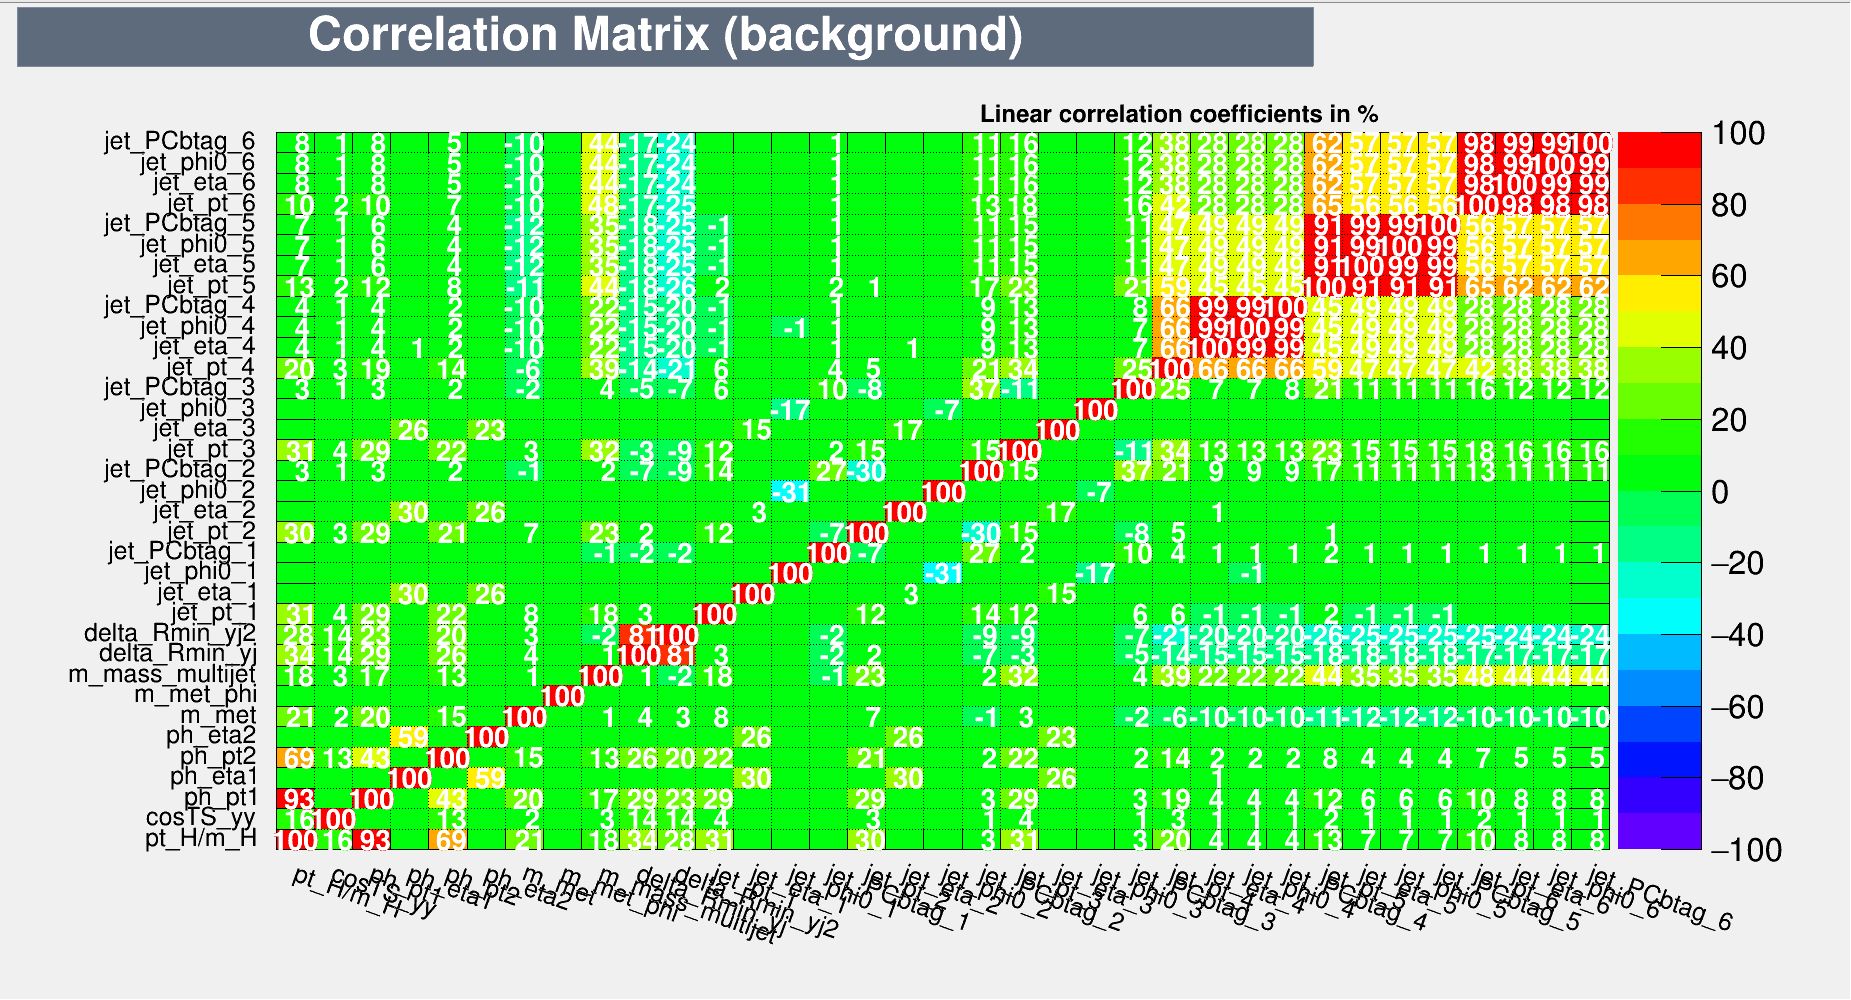
\includegraphics[width=0.62\textwidth]{figures/TMVABDTStudies/had-vbls4vec/had4veccorrMatEven.png}}\\
	\subfloat[CP Odd $ttH$]{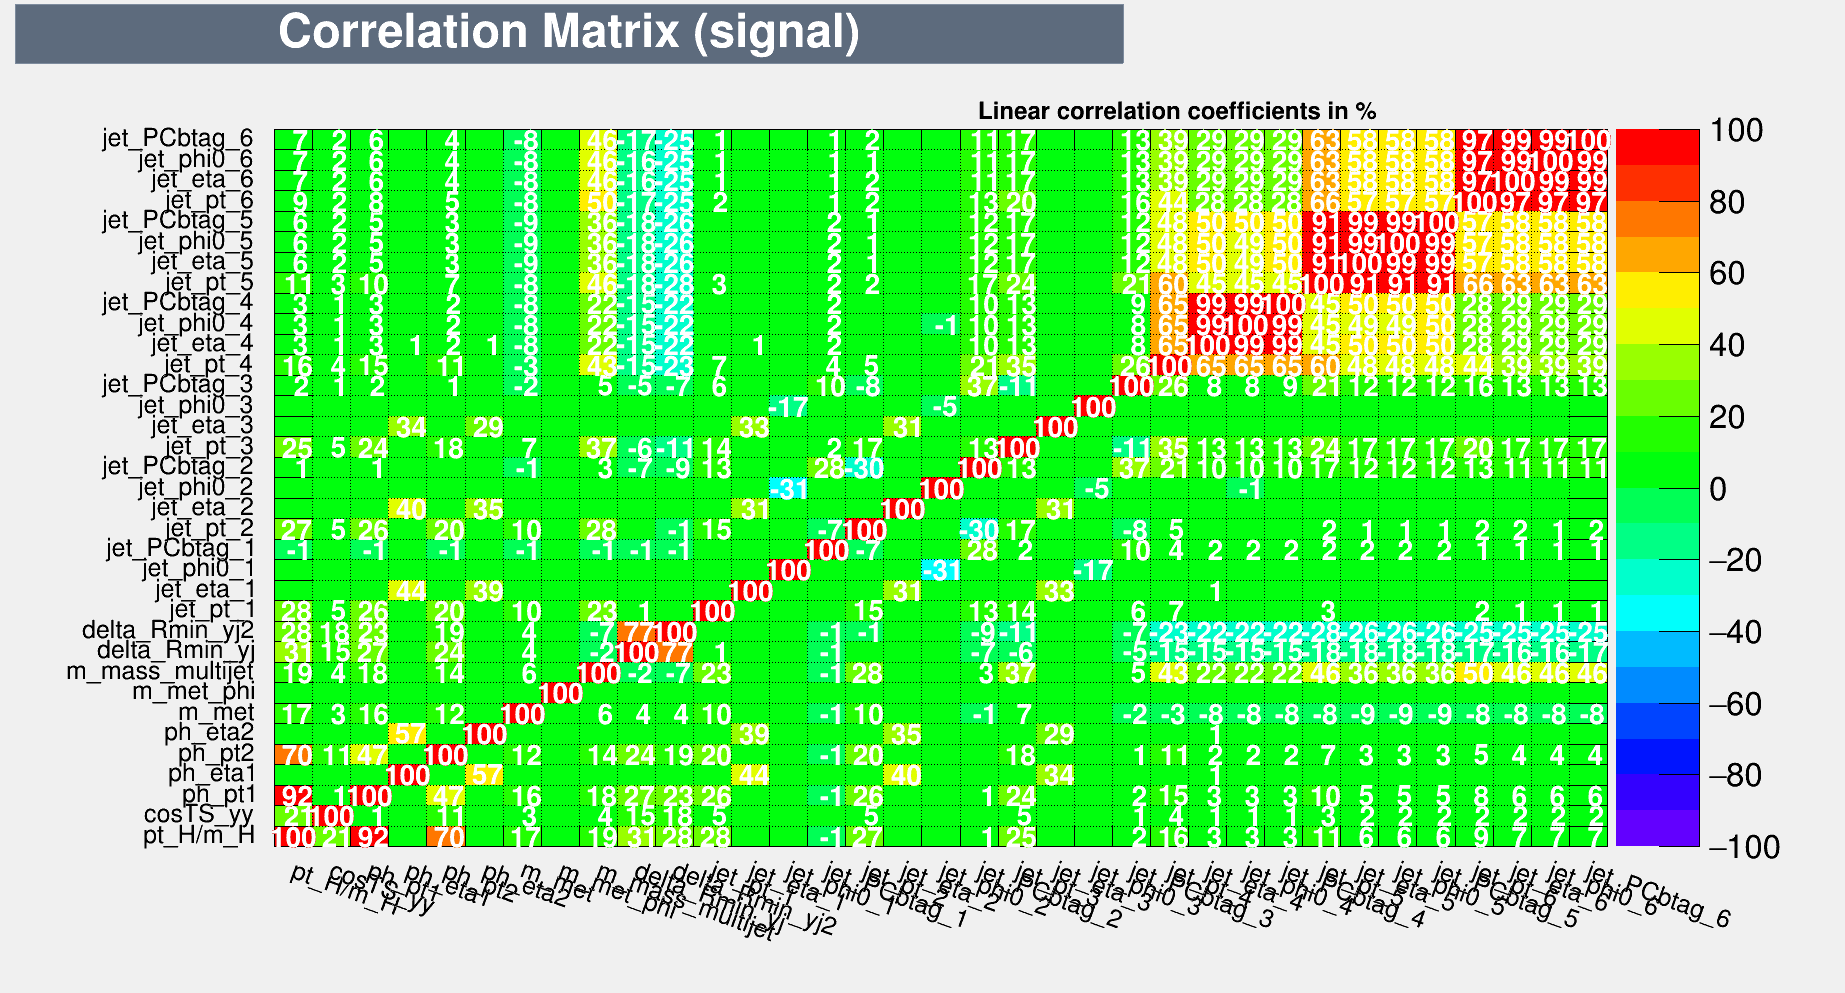
\includegraphics[width=0.62\textwidth]{figures/TMVABDTStudies/had-vbls4vec/had4veccorrMatOdd.png}} 
  \caption{Training variable correlations for events passing hadronic pre-selection.}
  \label{fig:hadcorr4vec}
\end{figure}

\begin{figure}[htbp]
  \centering
  	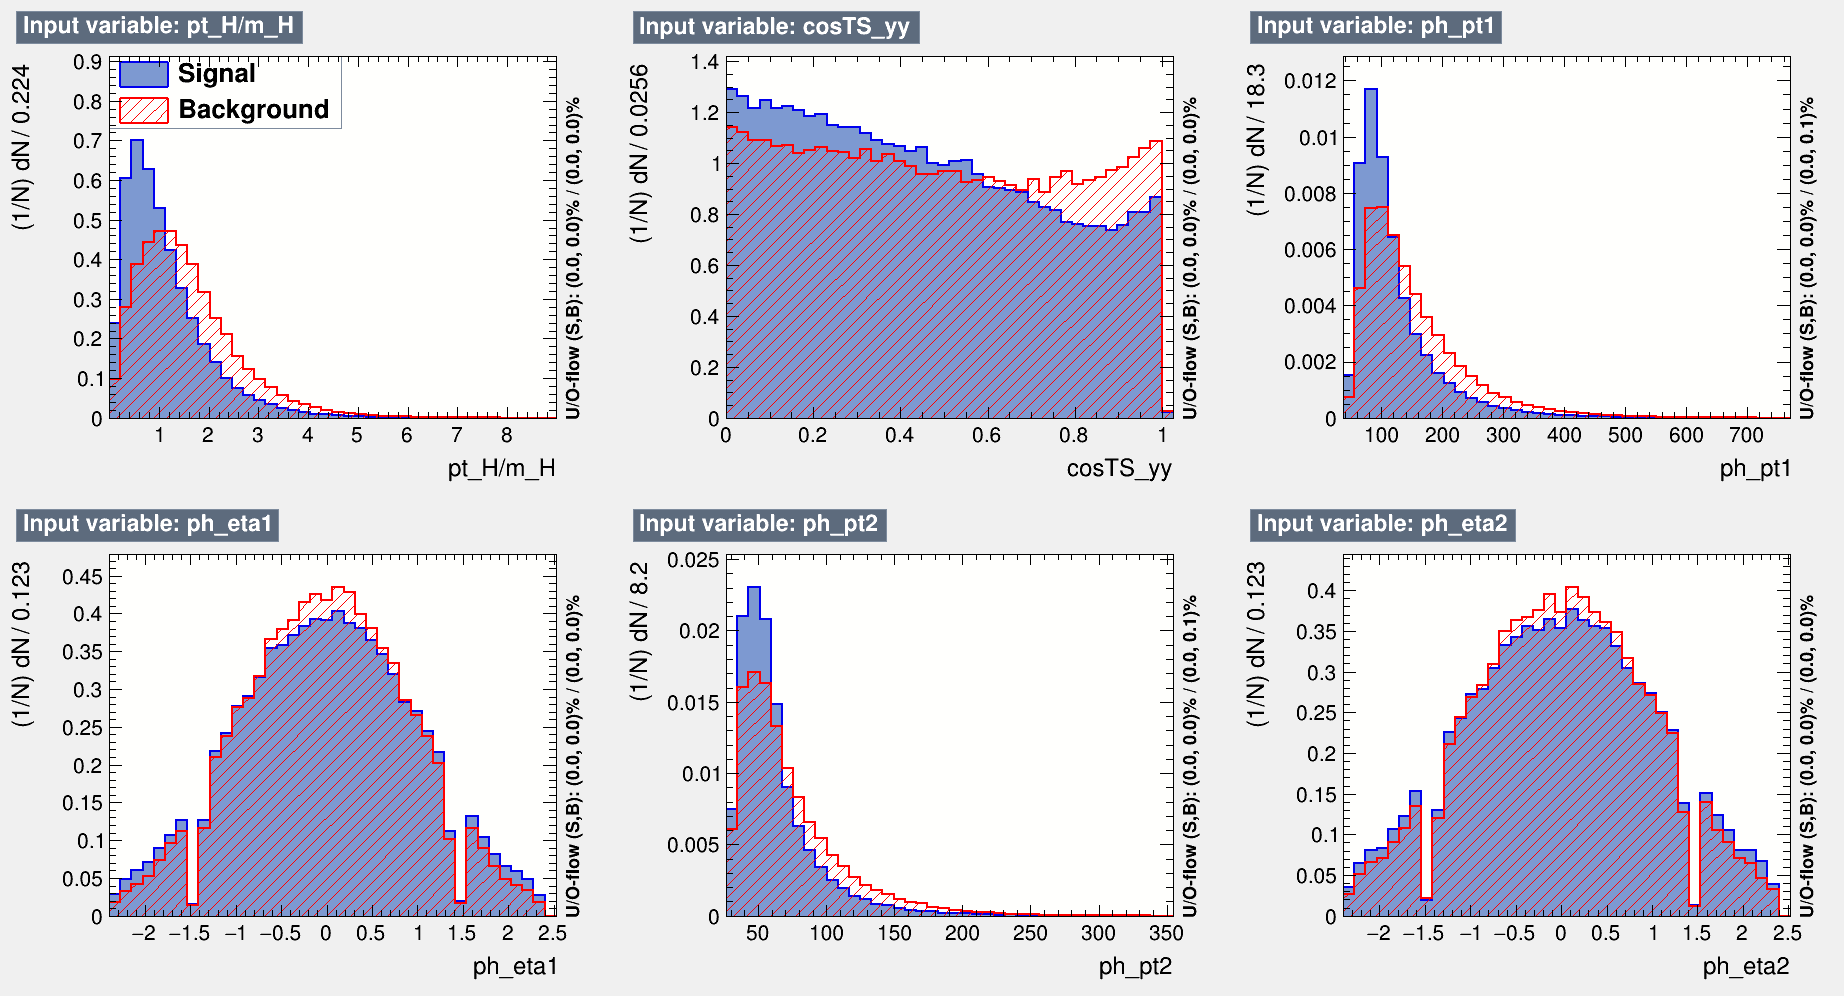
\includegraphics[width=0.62\textwidth]{figures/TMVABDTStudies/had-vbls4vec/had4vecvbls1.png}
  \caption{Normalized training variables for the 4-vector BDT, output by TMVA. CP-odd ttH is denoted as "signal" (blue); CP-even ttH is denoted as "background" (red). Variables shown are, from left to right, top row to bottom row: Higgs candidate $p_{T}$ (scaled by mass), $\cos$($\theta^{*}$), leading photon $p_{T}$, leading photon $\eta$, subleading photon $p_{T}$, and subleading photon $\eta$.}
  \label{fig:had4vecvbls1}
\end{figure}

\begin{figure}[htbp]
  \centering
  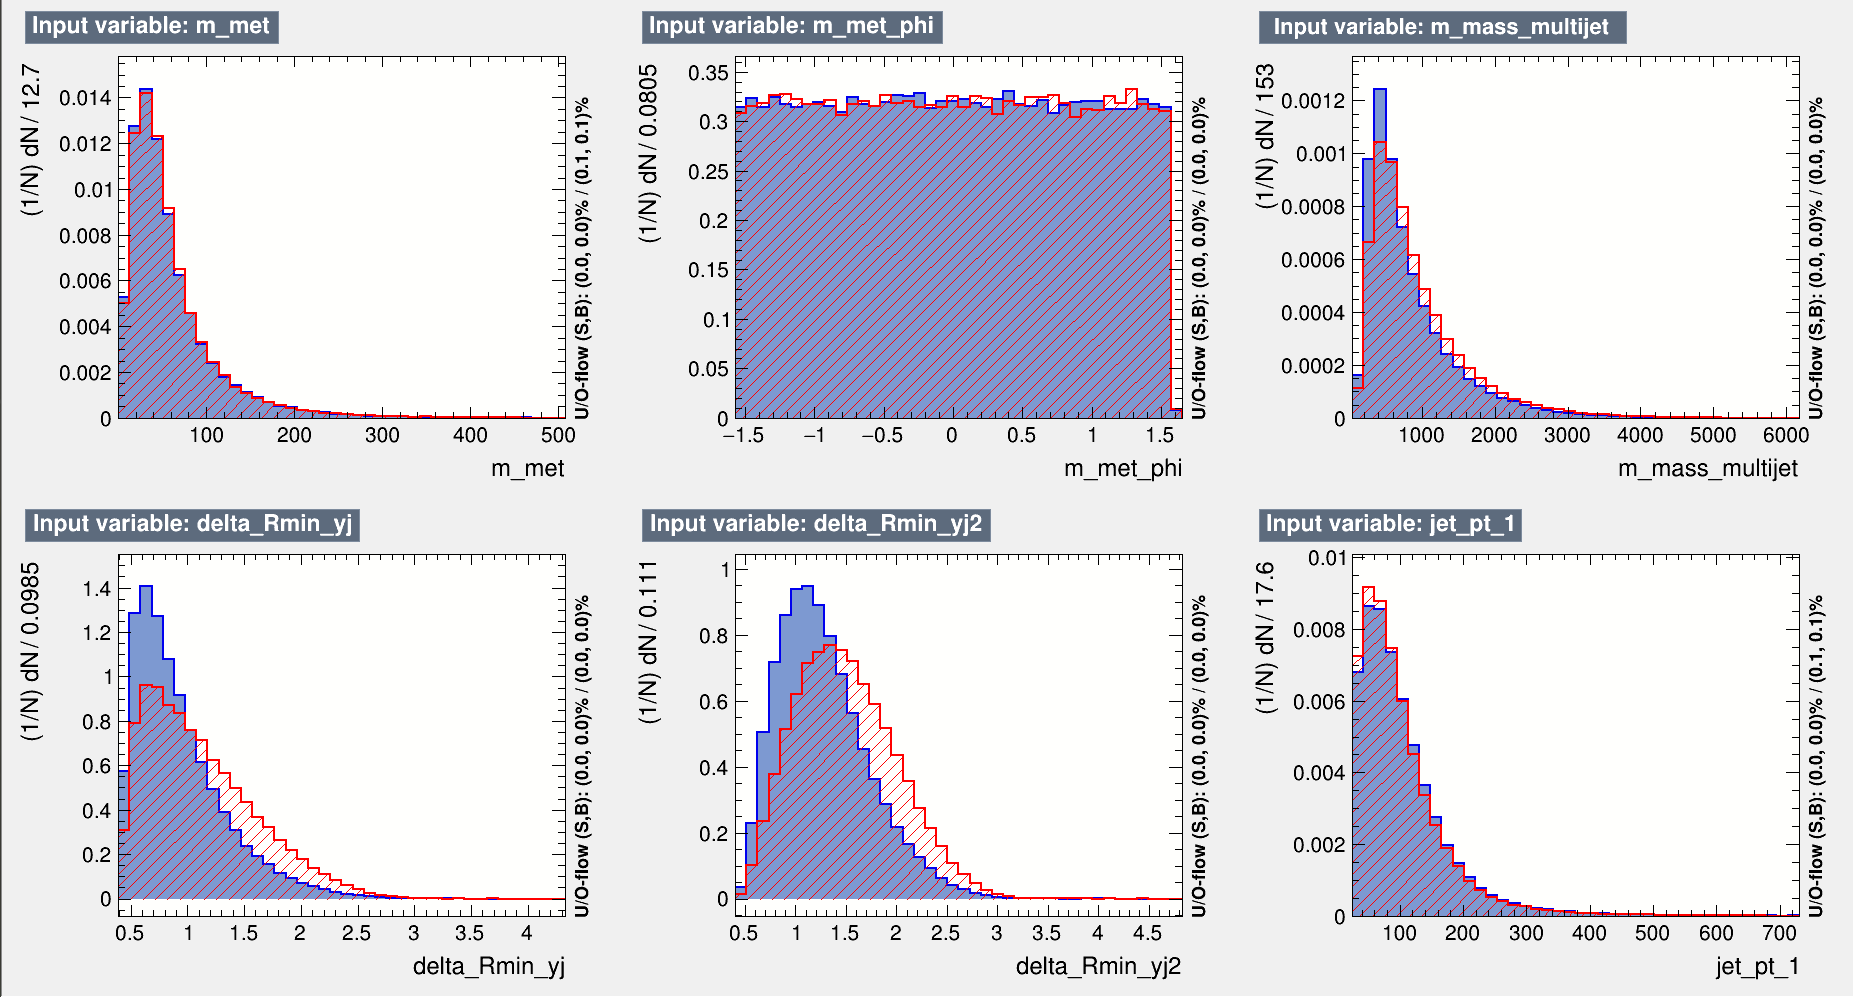
\includegraphics[width=0.62\textwidth]{figures/TMVABDTStudies/had-vbls4vec/had4vecvbls2.png}
  \caption{Normalized training variables for the 4-vector BDT, output by TMVA. CP-odd ttH is denoted as "signal" (blue); CP-even ttH is denoted as "background" (red). Variables shown are, from left to right, top row to bottom row: Magnitude of MET, MET $\phi$ (branch cut chosen to range from -$\pi$/2 to $\pi$/2), invariant mass of all jets in the event, minimum $\Delta$R between a photon and a jet, second-smallest $\Delta$R between a photon and a jet, $p_{T}$ of highest b-tag scoring jet.}
  \label{fig:had4vecvbls2}
\end{figure}

\begin{figure}[htbp]
  \centering
  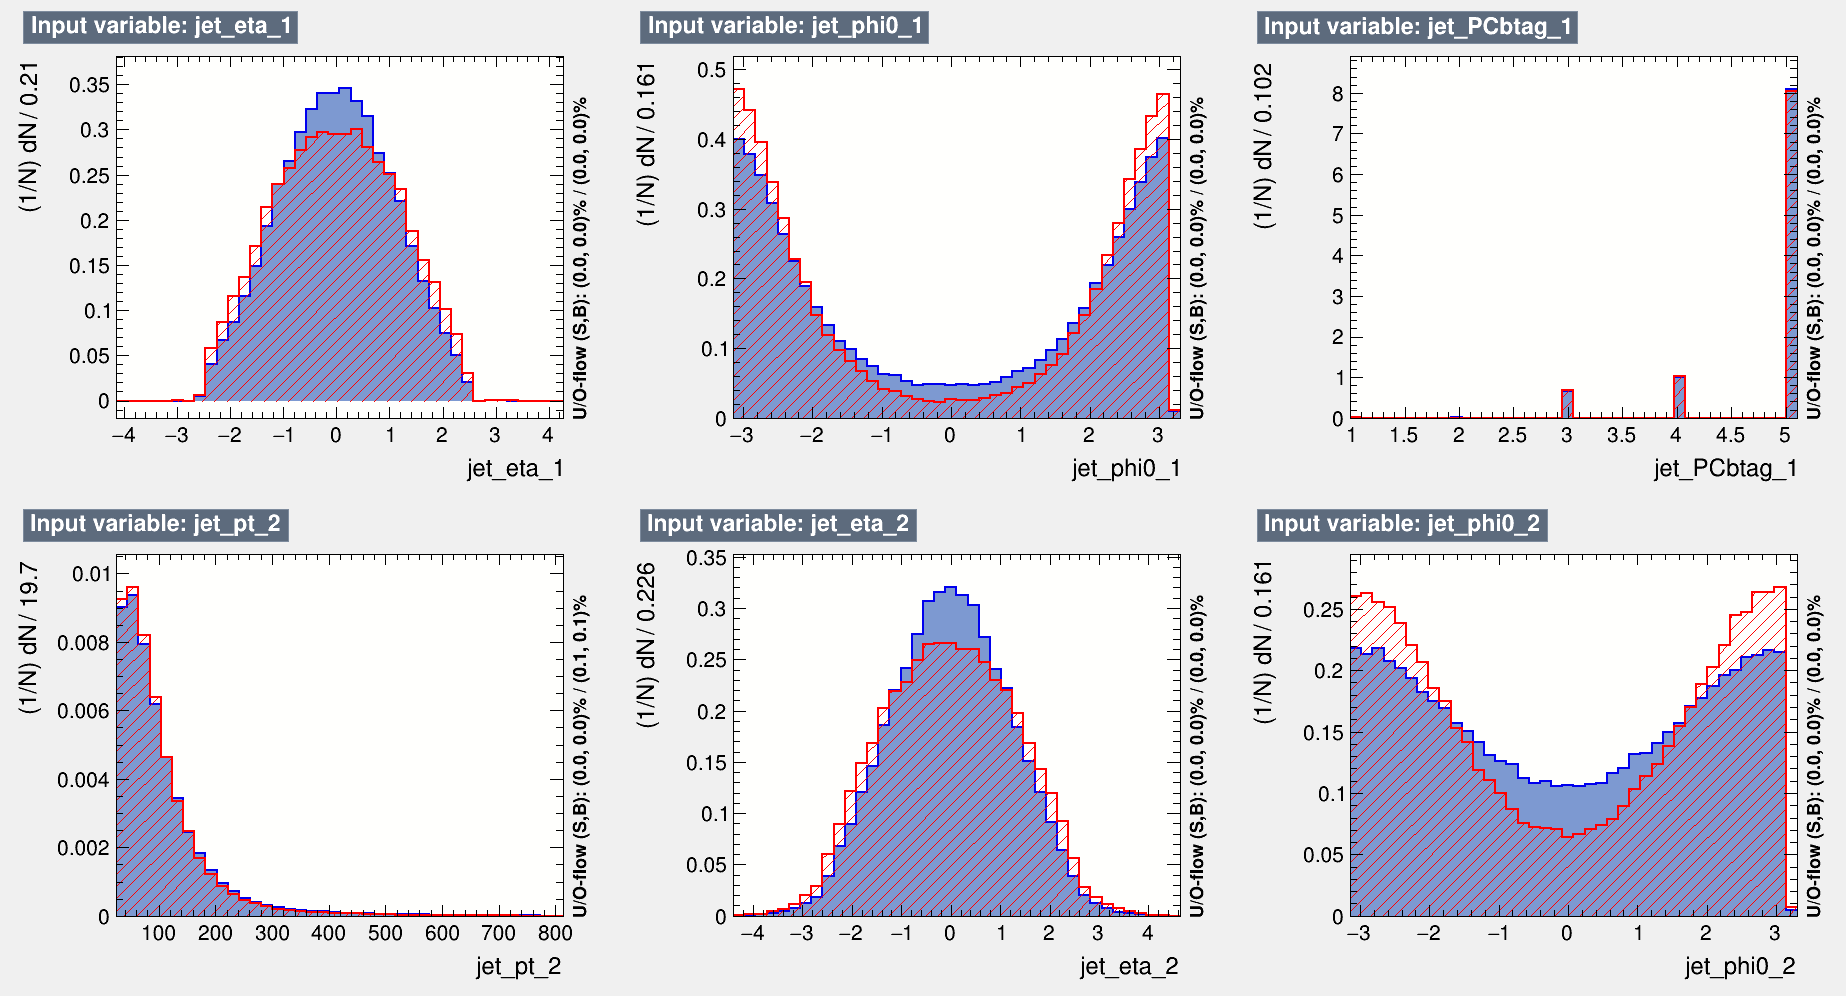
\includegraphics[width=0.62\textwidth]{figures/TMVABDTStudies/had-vbls4vec/had4vecvbls3.png}
  \caption{Normalized training variables for the 4-vector BDT, output by TMVA. CP-odd ttH is denoted as "signal" (blue); CP-even ttH is denoted as "background" (red). Variables shown are, from left to right, top row to bottom row: $\eta$ of highest b-tag scoring jet, $\phi$ of highest btag-scoring jet (measured with respect to the Higgs candidate), pseudo-continuous b-tag score of highest btag-scoring jet, $p_{T}$ of second-highest b-tag scoring jet, $\eta$ of second-highest b-tag scoring jet, $\phi$ of second-highest btag-scoring jet (measured with respect to the Higgs candidate).}
  \label{fig:had4vecvbls3}
\end{figure}

\begin{figure}[htbp]
  \centering
  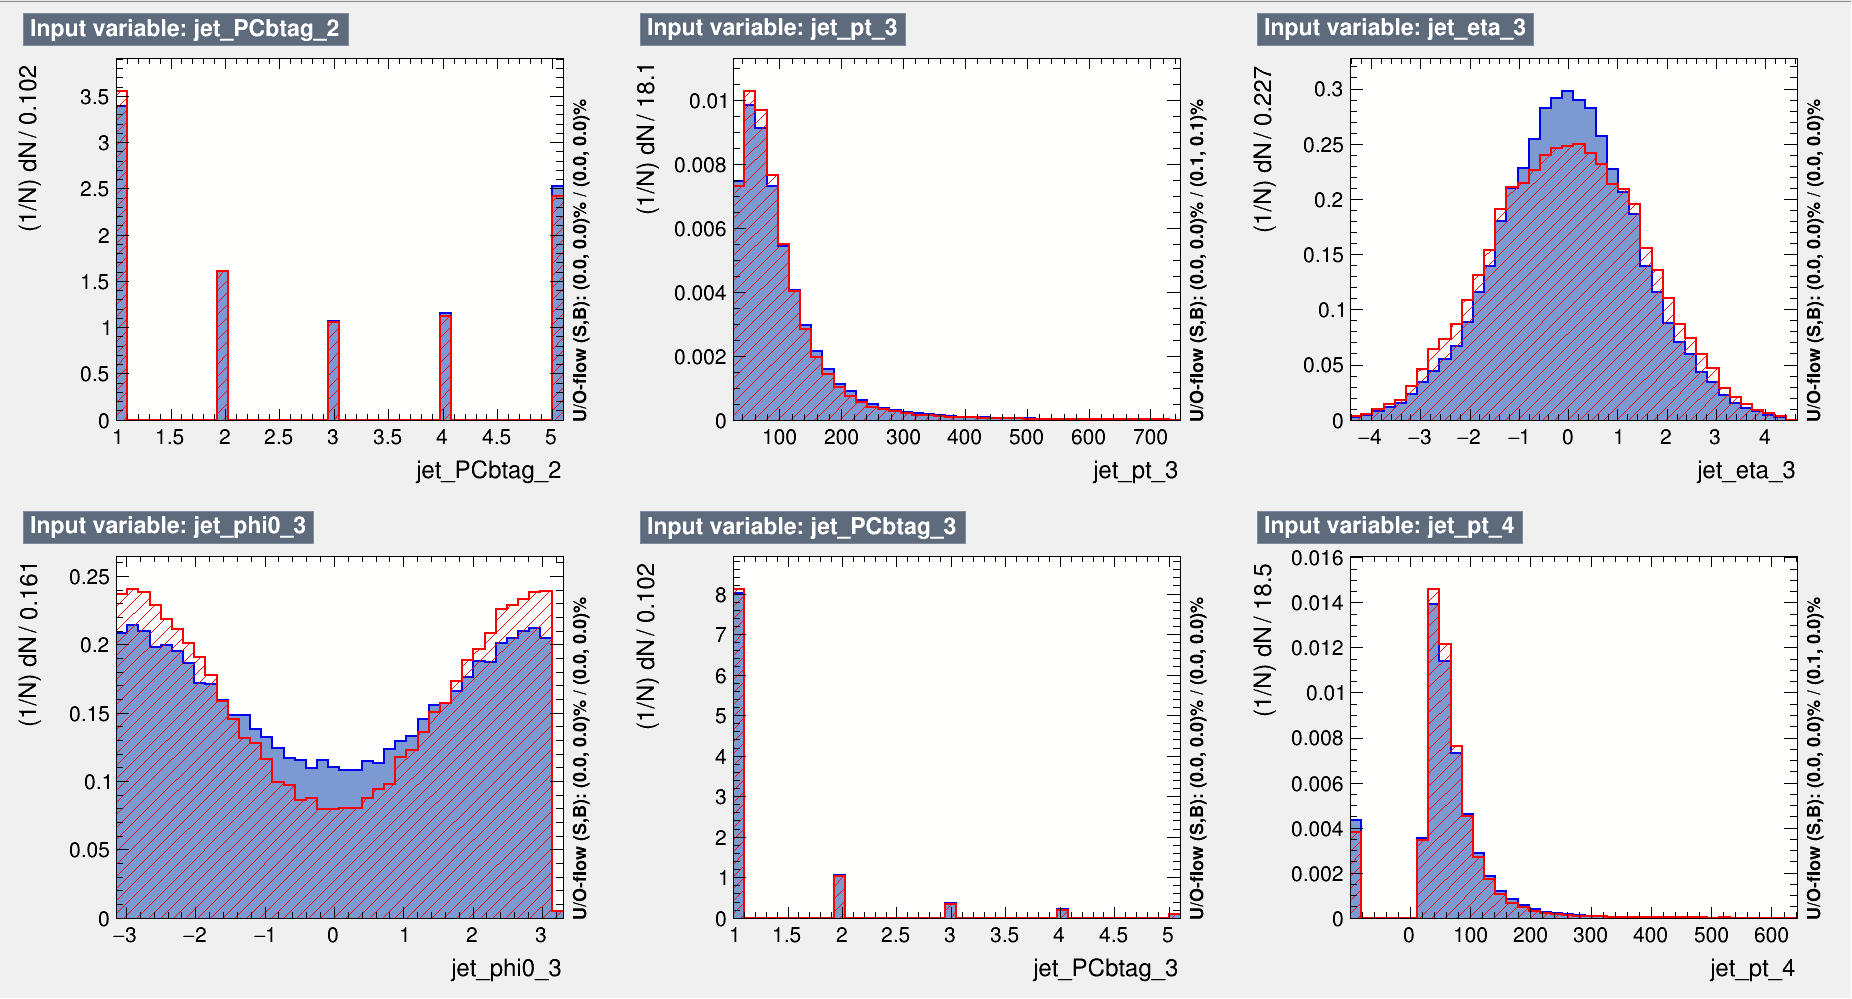
\includegraphics[width=0.62\textwidth]{figures/TMVABDTStudies/had-vbls4vec/had4vecvbls4.png}
  \caption{Normalized training variables for the 4-vector BDT, output by TMVA. CP-odd ttH is denoted as "signal" (blue); CP-even ttH is denoted as "background" (red). Variables shown are, from left to right, top row to bottom row: pseudo-continuous b-tag score of second-highest btag-scoring jet, $p_{T}$ of third-highest b-tag scoring jet, $\eta$ of third-highest b-tag scoring jet, $\phi$ of third-highest btag-scoring jet (measured with respect to the Higgs candidate), pseudo-continuous b-tag score of third-highest btag-scoring jet, $p_{T}$ of fourth-highest b-tag scoring jet.}
  \label{fig:had4vecvbls4}
\end{figure}

\begin{figure}[htbp]
  \centering
  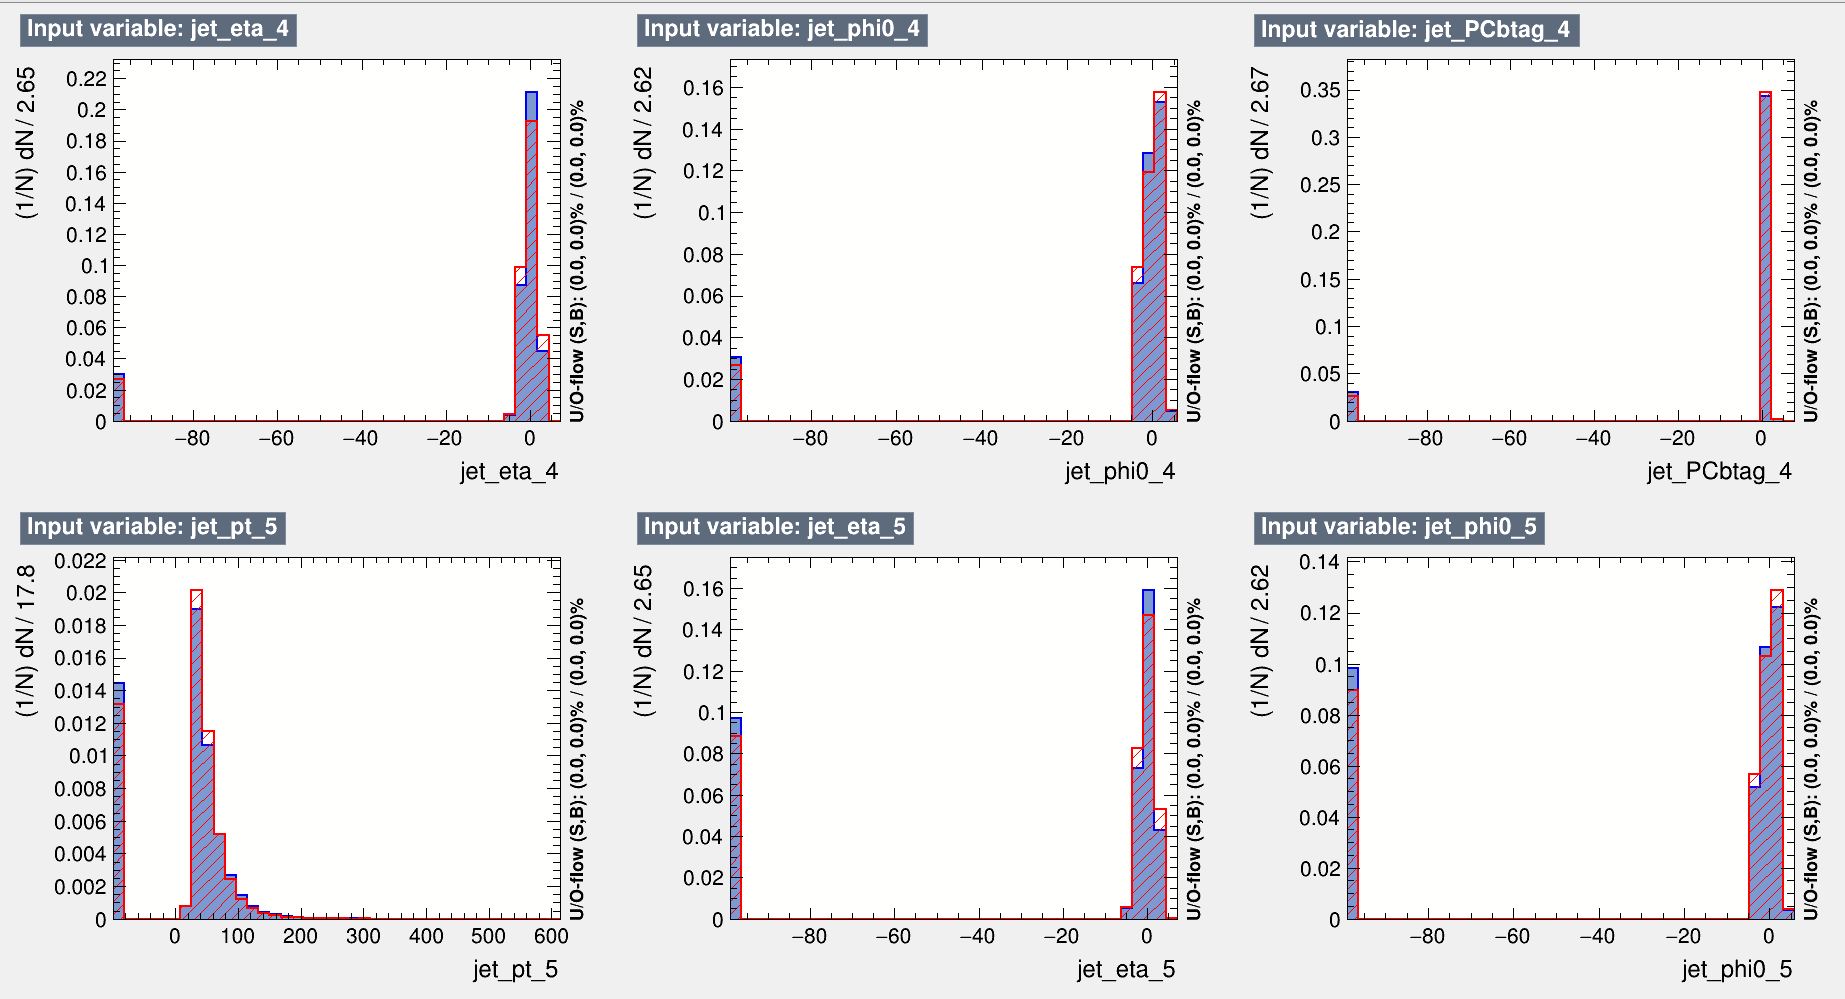
\includegraphics[width=0.62\textwidth]{figures/TMVABDTStudies/had-vbls4vec/had4vecvbls5.png}
  \caption{Normalized training variables for the 4-vector BDT, output by TMVA. CP-odd ttH is denoted as "signal" (blue); CP-even ttH is denoted as "background" (red). Variables shown are, from left to right, top row to bottom row: $\eta$ of fourth-highest b-tag scoring jet, $\phi$ of fourth-highest btag-scoring jet (measured with respect to the Higgs candidate), pseudo-continuous b-tag score of fourth-highest btag-scoring jet, $p_{T}$ of fifth-highest b-tag scoring jet, $\eta$ of fifth-highest b-tag scoring jet, $\phi$ of fifth-highest btag-scoring jet (measured with respect to the Higgs candidate)}
  \label{fig:had4vecvbls5}
\end{figure}
  
\begin{figure}[htbp]
  \centering
  	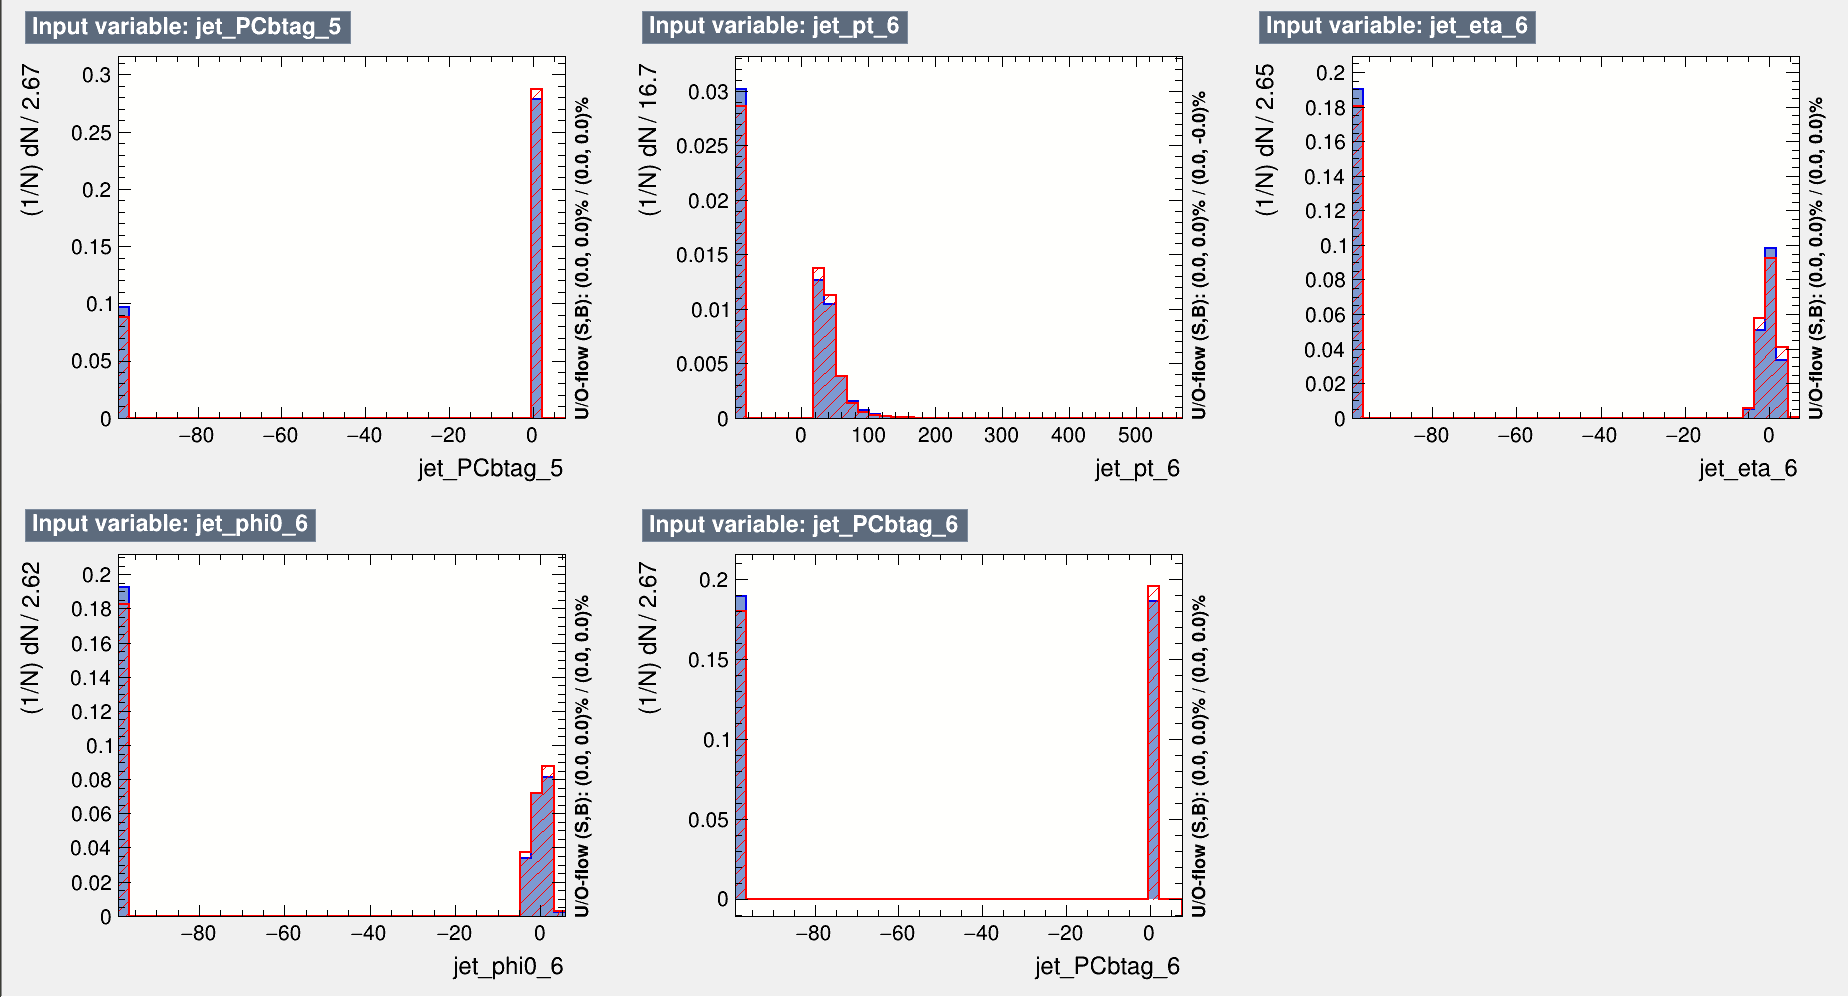
\includegraphics[width=0.62\textwidth]{figures/TMVABDTStudies/had-vbls4vec/had4vecvbls6.png}
  \caption{Normalized training variables for the 4-vector BDT, output by TMVA. CP-odd ttH is denoted as "signal" (blue); CP-even ttH is denoted as "background" (red). Variables shown are, from left to right, top row to bottom row: Pseudo-continuous b-tag score of fifth-highest btag-scoring jet, $p_{T}$ of sixth-highest b-tag scoring jet, $\eta$ of sixth-highest b-tag scoring jet, $\phi$ of sixth-highest btag-scoring jet (measured with respect to the Higgs candidate), pseudo-continuous b-tag score of sixth-highest btag-scoring jet.}
  \label{fig:had4vecvbls6}
  
\end{figure}

\clearpage

\subsubsection{Leptonic channel}

Likewise, the leptonic  four-vector CP BDT is trained to separate $ttH$ CP even and CP odd aMCnlo+Pythia8 Monte Carlo passing the leptonic pre-selection (>0 leptons, $\ge1$ b-jet at 77\% working point).

\begin{itemize}
\item $p_{T}$, $\eta$, $\phi$, and pseudocontinuous b-tag score of the leading 4 jets in the event
\item $p_{T}$, $\eta$, $\phi$, and pseudocontinuous b-tag score of the leading 2 leptons in the event
\item The $p_{T}$ of the Higgs candidate (scaled by mass)
\item  $\cos$($\theta^{*}$) (the cosine of the angle between the photons in the Collins-Soper frame \ref{cite:thetastar})
\item The $\eta$ and $\phi$ of the two leading photons in the event
\item The magnitude and $\phi$ of the missing transverse energy in the event
\item The summed invariant mass of all jets in the event
\item The minimum $\Delta$R between a photon and a jet in the event
\item The second-smallest $\Delta$R between a photon and a jet in the event
\end{itemize} 

The linear correlations between these variables in $ttH$ CP even and CP odd aMCnlo+Pythiya8 Monte Carlo are shown in Figure \ref{fig:lepcorr4vec}.  Figures \ref{fig:lep4vecvbls1} - \ref{fig:lep4vecvbls6} compare the distribution of each training variable in $ttH$ CP even and CP odd Monte Carlo.

\begin{figure}[htbp]
  \centering
    \subfloat[CP Even $ttH$]{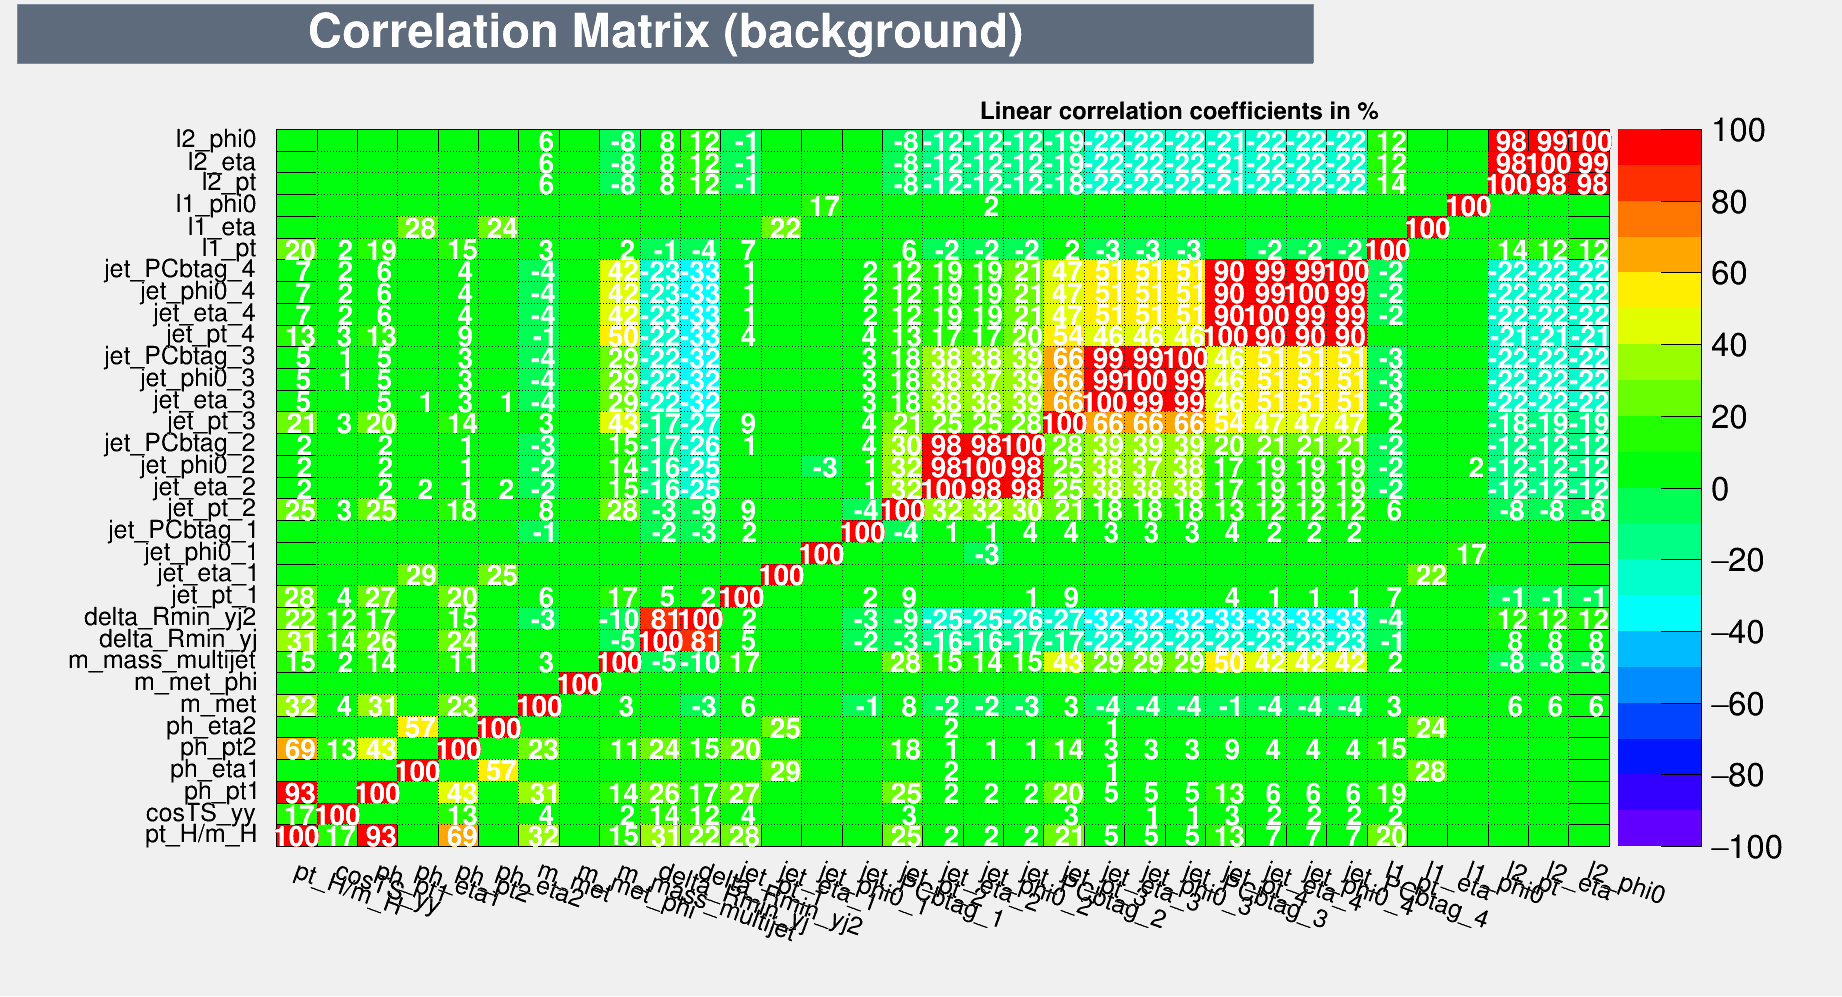
\includegraphics[width=0.62\textwidth]{figures/TMVABDTStudies/lep-vbls4vec/lep4veccorrMatEven.png}}\\
	\subfloat[CP Odd $ttH$]{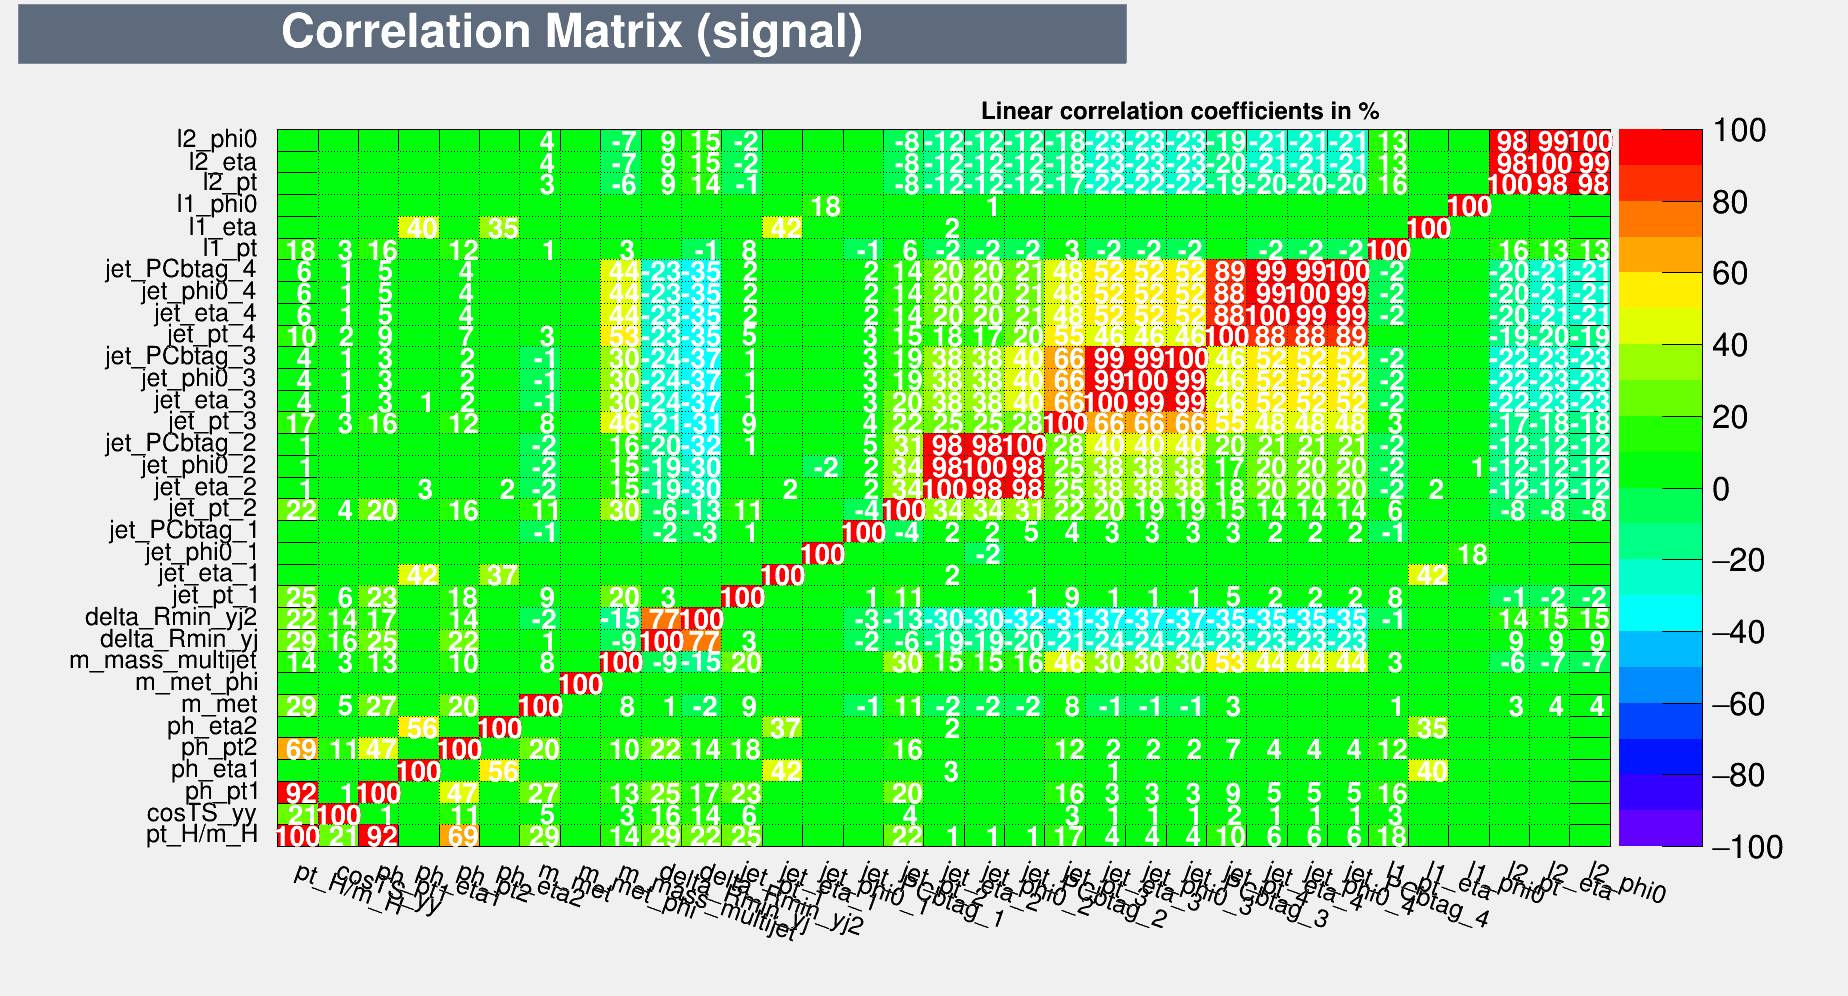
\includegraphics[width=0.62\textwidth]{figures/TMVABDTStudies/lep-vbls4vec/lep4veccorrMatOdd.png}} 
 \caption{Training variable correlations for events passing leptonic pre-selection.}
  \label{fig:lepcorr4vec}
\end{figure}

\begin{figure}[htbp]
  \centering
  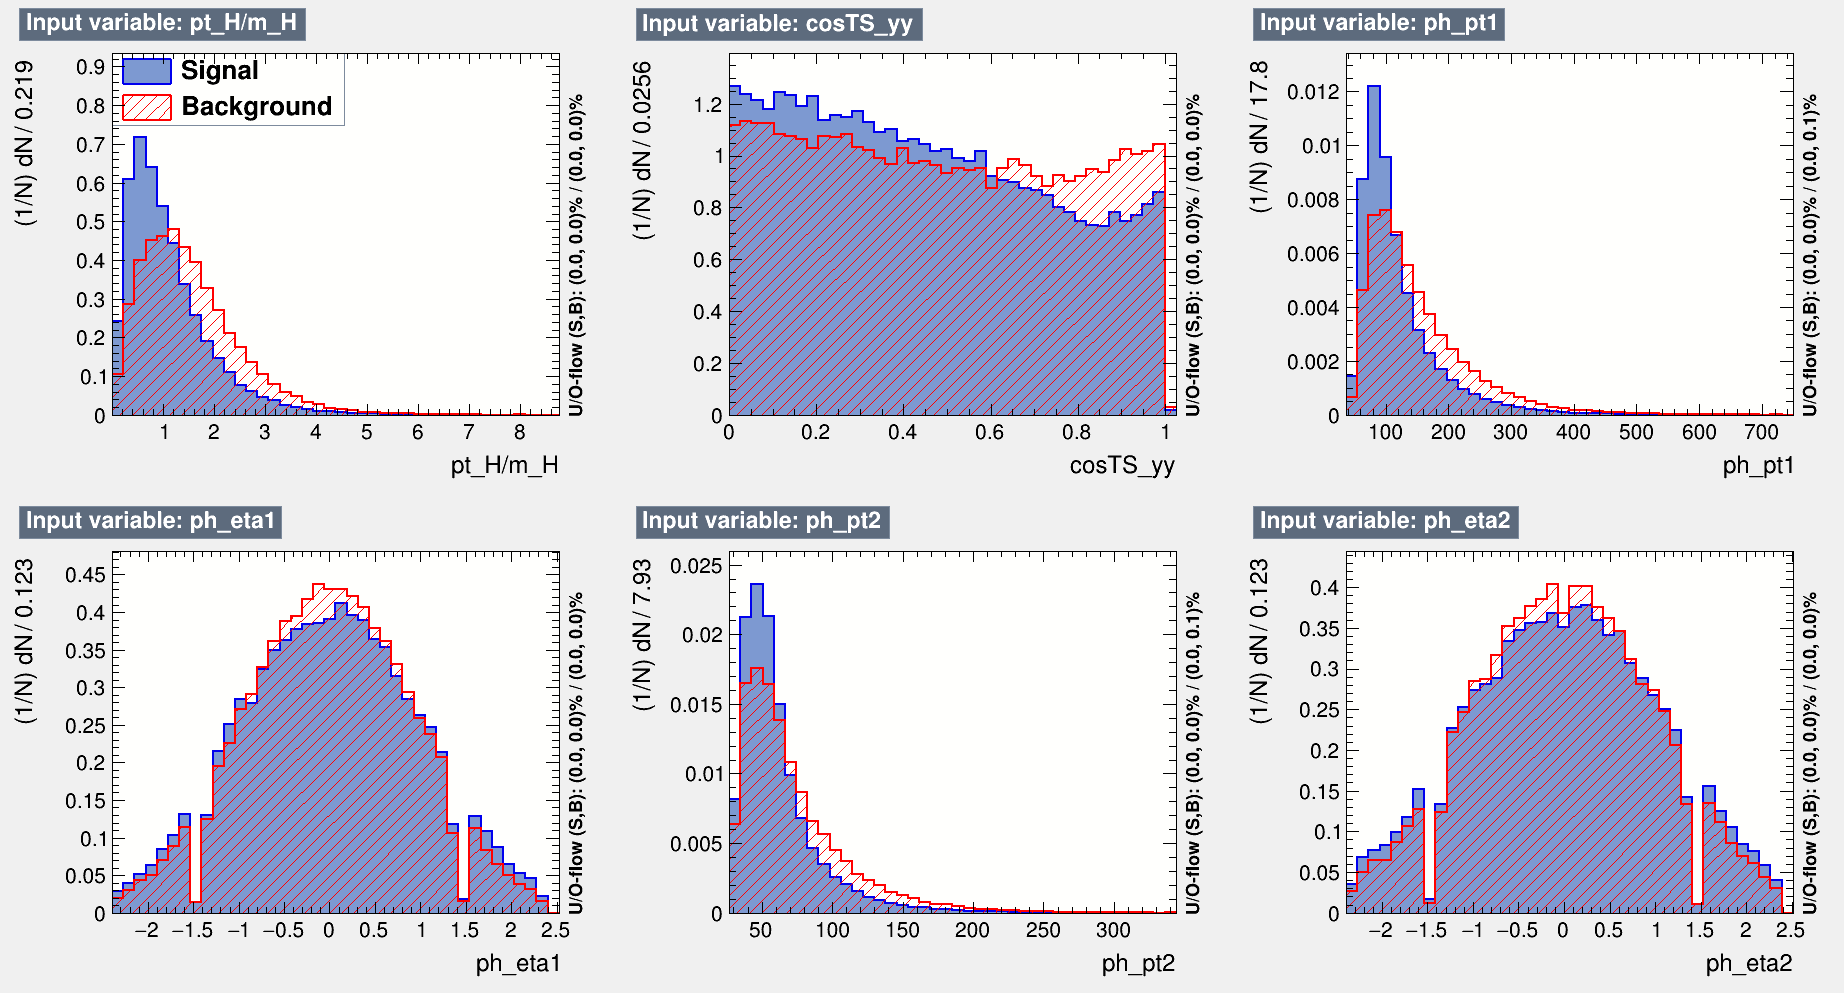
\includegraphics[width=0.62\textwidth]{figures/TMVABDTStudies/lep-vbls4vec/lep4vecvbls1.png}
  \caption{Normalized training variables for the 4-vector BDT, output by TMVA. CP-odd ttH is denoted as "signal" (blue); CP-even ttH is denoted as "background" (red). Variables shown are, from left to right, top row to bottom row: Higgs candidate $p_{T}$ (scaled by mass), $\cos$($\theta^{*}$), leading photon $p_{T}$, leading photon $\eta$, subleading photon $p_{T}$, and subleading photon $\eta$.}
  \label{fig:lep4vecvbls1}
\end{figure}

\begin{figure}[htbp]
  \centering
  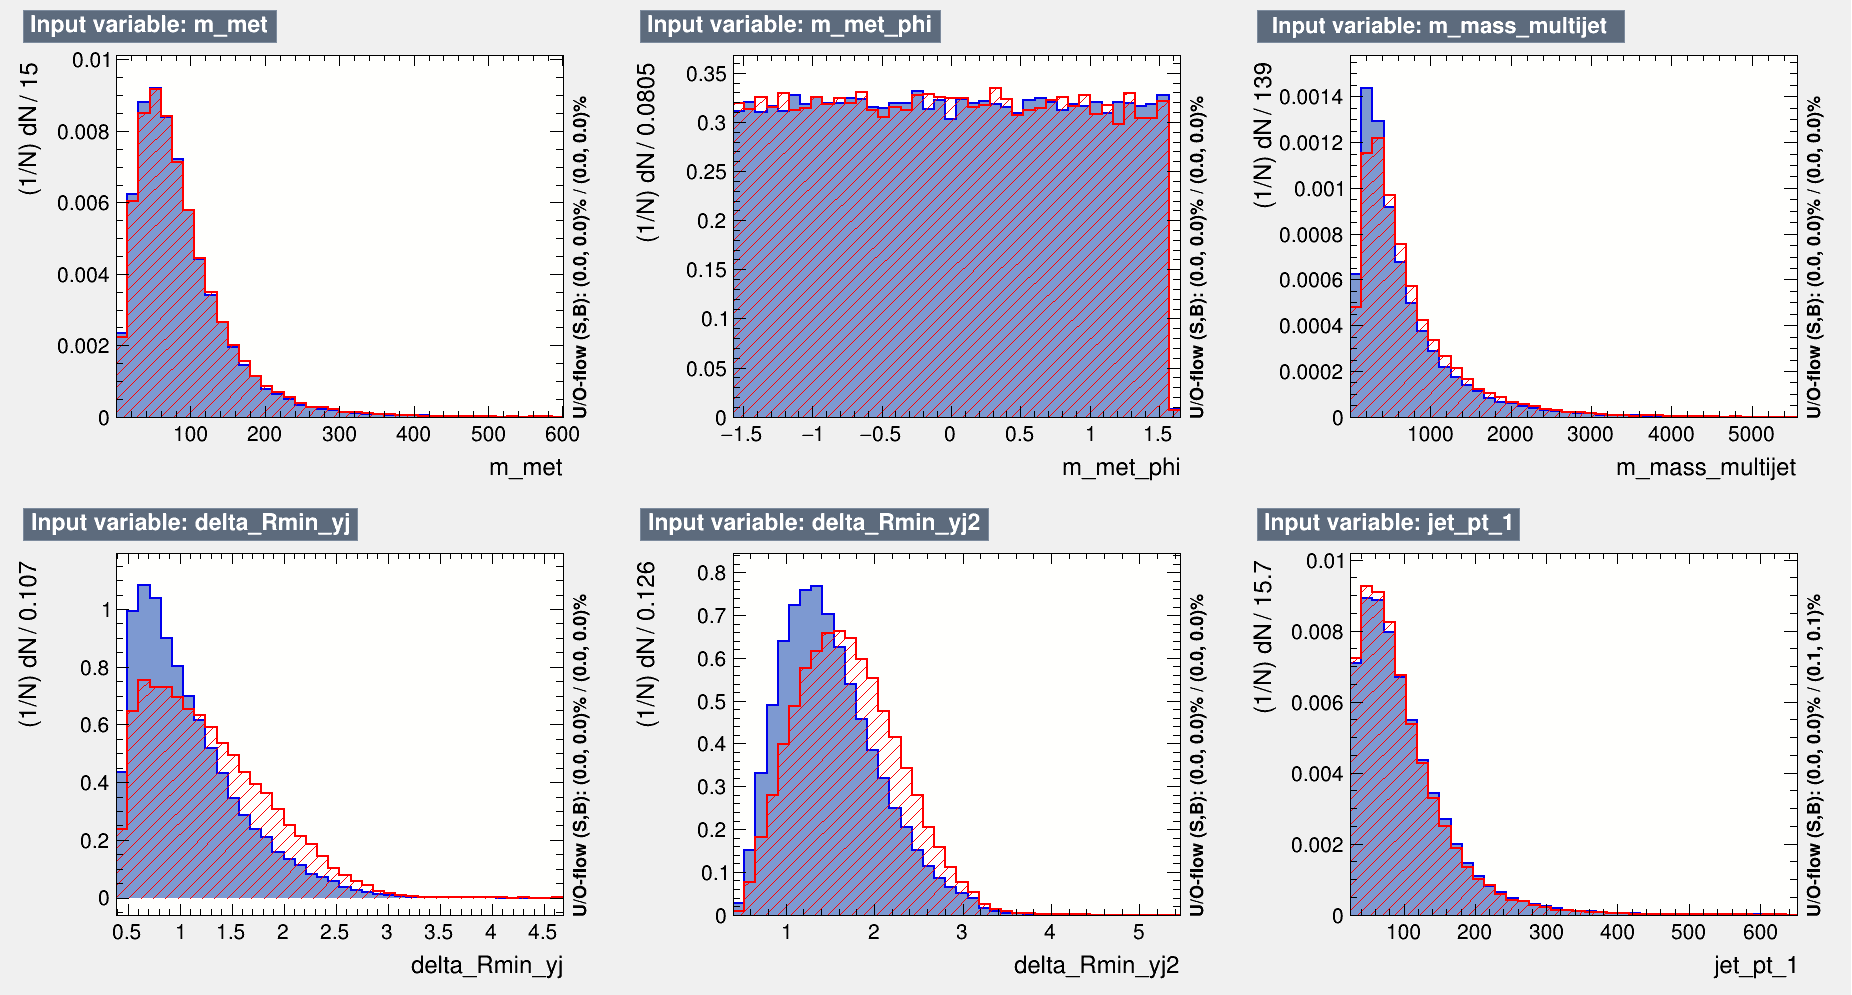
\includegraphics[width=0.62\textwidth]{figures/TMVABDTStudies/lep-vbls4vec/lep4vecvbls2.png}
  \caption{Normalized training variables for the 4-vector BDT, output by TMVA. CP-odd ttH is denoted as "signal" (blue); CP-even ttH is denoted as "background" (red). Variables shown are, from left to right, top row to bottom row: Magnitude of MET, MET $\phi$ (branch cut chosen to range from -$\pi$/2 to $\pi$/2), invariant mass of all jets in the event, minimum $\Delta$R between a photon and a jet, second-smallest $\Delta$R between a photon and a jet, $p_{T}$ of highest b-tag scoring jet.}
  \label{fig:lep4vecvbls2}
\end{figure}

\begin{figure}[htbp]
  \centering
  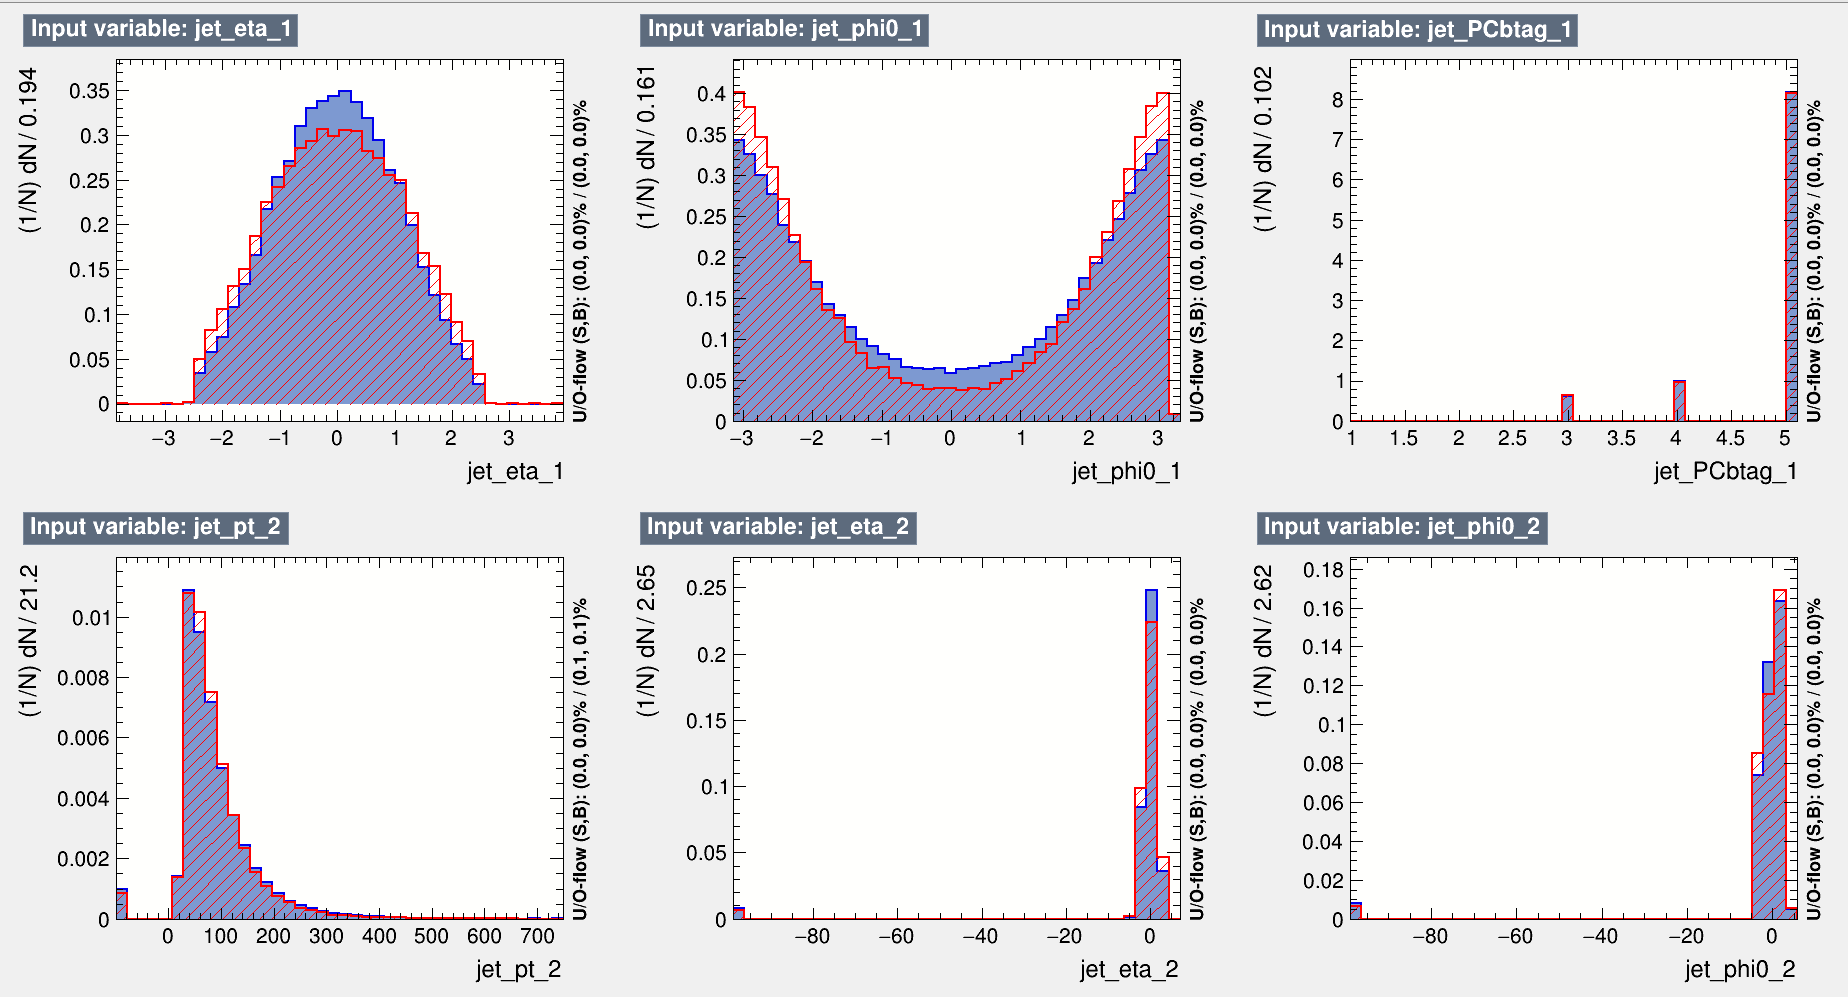
\includegraphics[width=0.62\textwidth]{figures/TMVABDTStudies/lep-vbls4vec/lep4vecvbls3.png}
  \caption{Normalized training variables for the 4-vector BDT, output by TMVA. CP-odd ttH is denoted as "signal" (blue); CP-even ttH is denoted as "background" (red). Variables shown are, from left to right, top row to bottom row: $\eta$ of highest b-tag scoring jet, $\phi$ of highest btag-scoring jet (measured with respect to the Higgs candidate), pseudo-continuous b-tag score of highest btag-scoring jet, $p_{T}$ of second-highest b-tag scoring jet, $\eta$ of second-highest b-tag scoring jet, $\phi$ of second-highest btag-scoring jet (measured with respect to the Higgs candidate).}
  \label{fig:lep4vecvbls3}
\end{figure}

\begin{figure}[htbp]
  \centering
  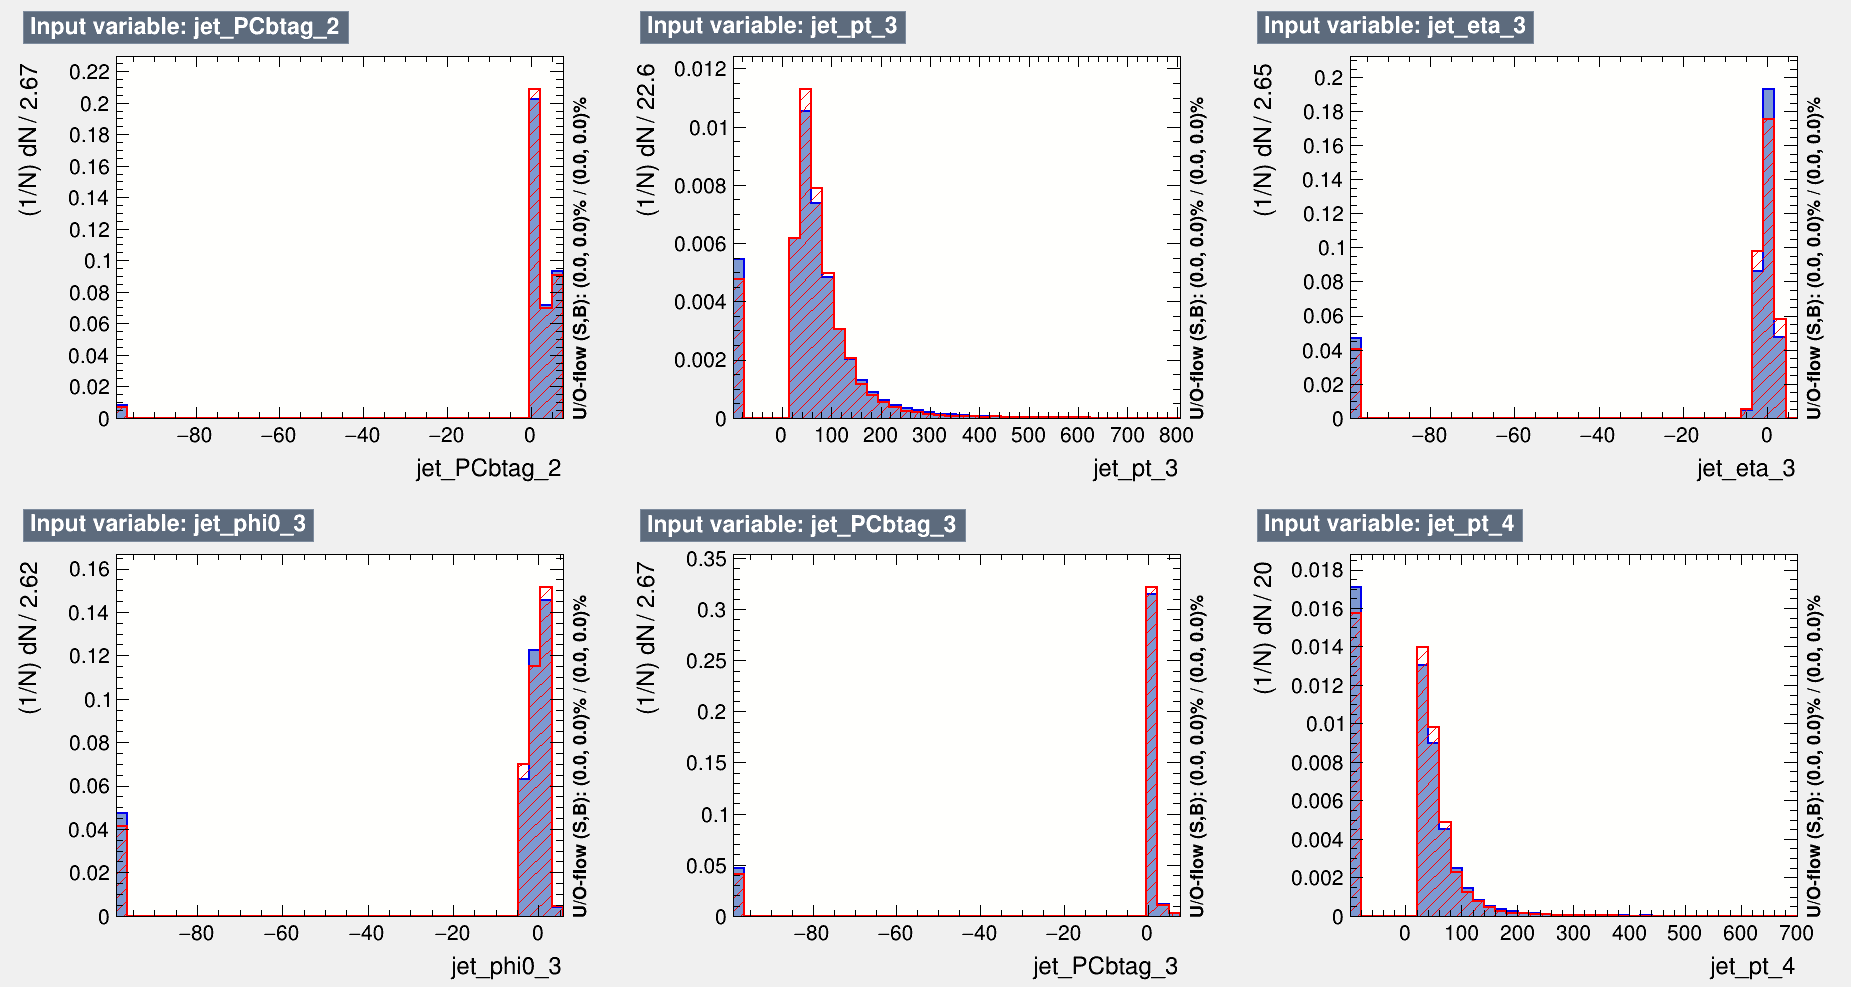
\includegraphics[width=0.62\textwidth]{figures/TMVABDTStudies/lep-vbls4vec/lep4vecvbls4.png}
  \caption{Normalized training variables for the 4-vector BDT, output by TMVA. CP-odd ttH is denoted as "signal" (blue); CP-even ttH is denoted as "background" (red). Variables shown are, from left to right, top row to bottom row: pseudo-continuous b-tag score of second-highest btag-scoring jet, $p_{T}$ of third-highest b-tag scoring jet, $\eta$ of third-highest b-tag scoring jet, $\phi$ of third-highest btag-scoring jet (measured with respect to the Higgs candidate), pseudo-continuous b-tag score of third-highest btag-scoring jet, $p_{T}$ of fourth-highest b-tag scoring jet.}
  \label{fig:lep4vecvbls4}
\end{figure}

\begin{figure}[htbp]
  \centering
  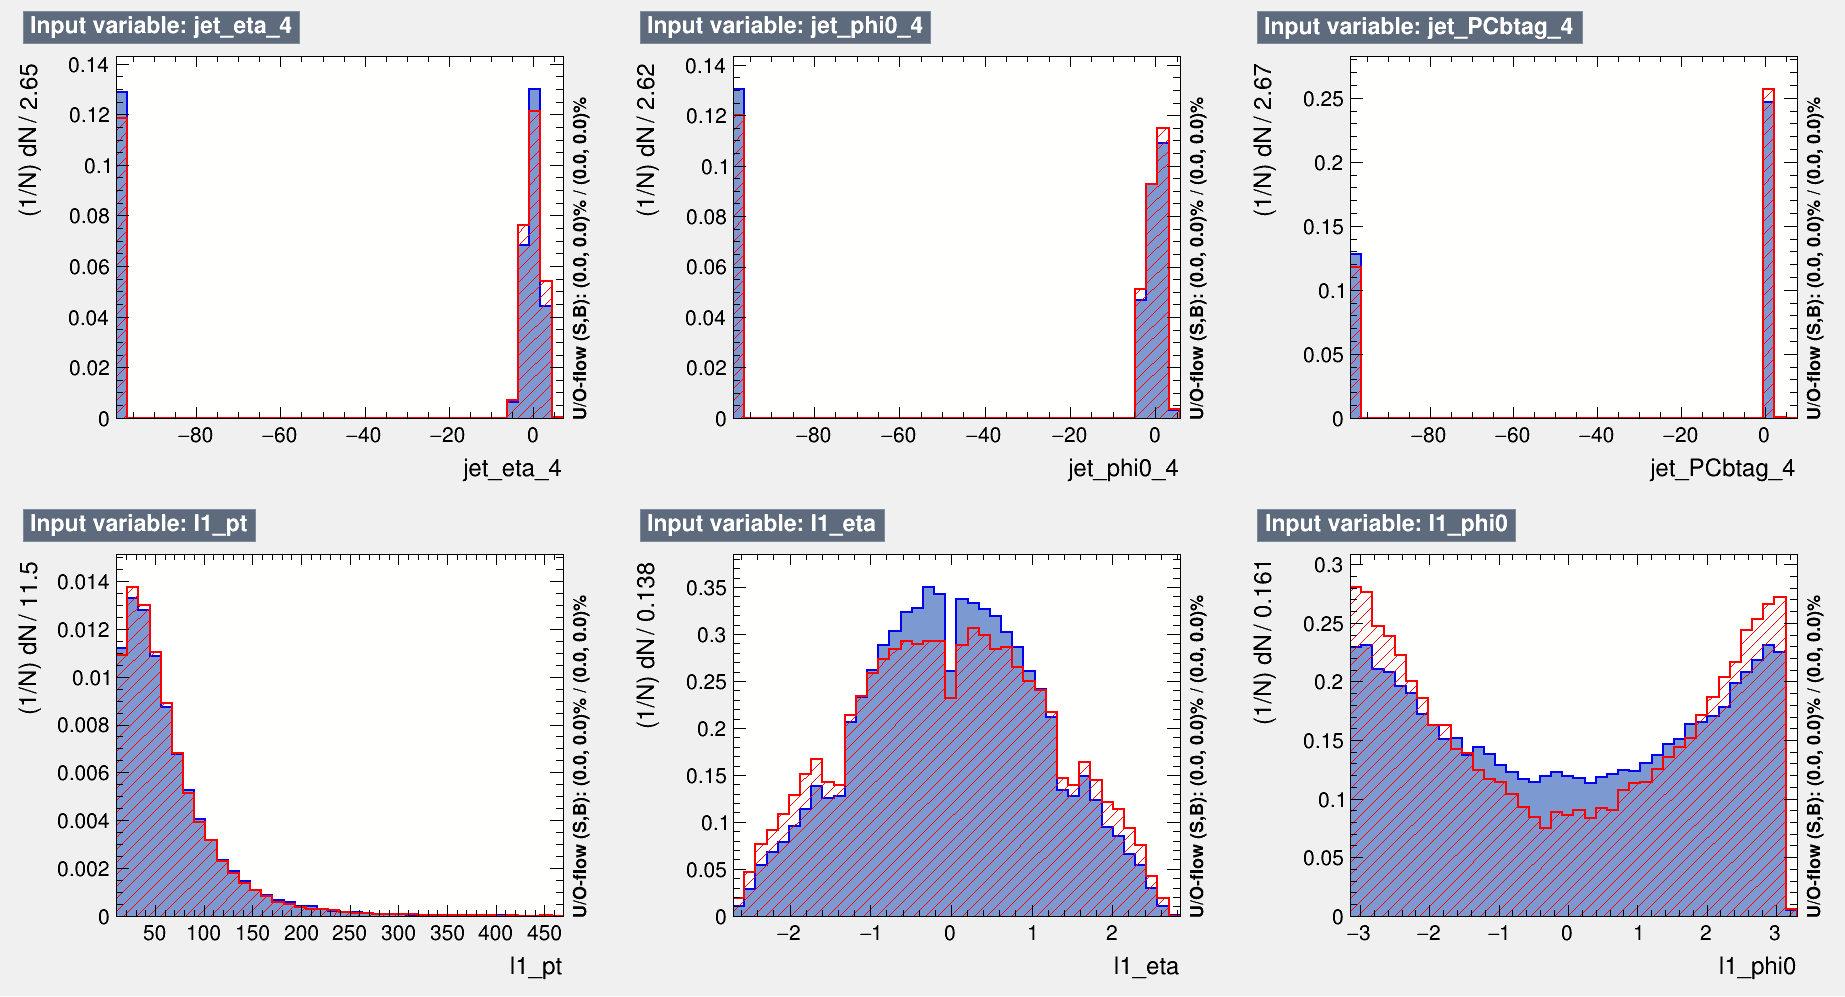
\includegraphics[width=0.62\textwidth]{figures/TMVABDTStudies/lep-vbls4vec/lep4vecvbls5.png}
  \caption{Normalized training variables for the 4-vector BDT, output by TMVA. CP-odd ttH is denoted as "signal" (blue); CP-even ttH is denoted as "background" (red). Variables shown are, from left to right, top row to bottom row: $\eta$ of fourth-highest btag-scoring jet, $\phi$ of fourth-highest btag-scoring jet (measured with respect to the Higgs candidate), pseudo-continuous b-tag score of fourth-highest btag-scoring jet, $p_{T}$ of leading lepton, $\eta$ of leading lepton, $\phi$ of leading lepton (measured with respect to the Higgs candidate).}
  \label{fig:lep4vecvbls5}
\end{figure}

\begin{figure}[htbp]
  \centering
  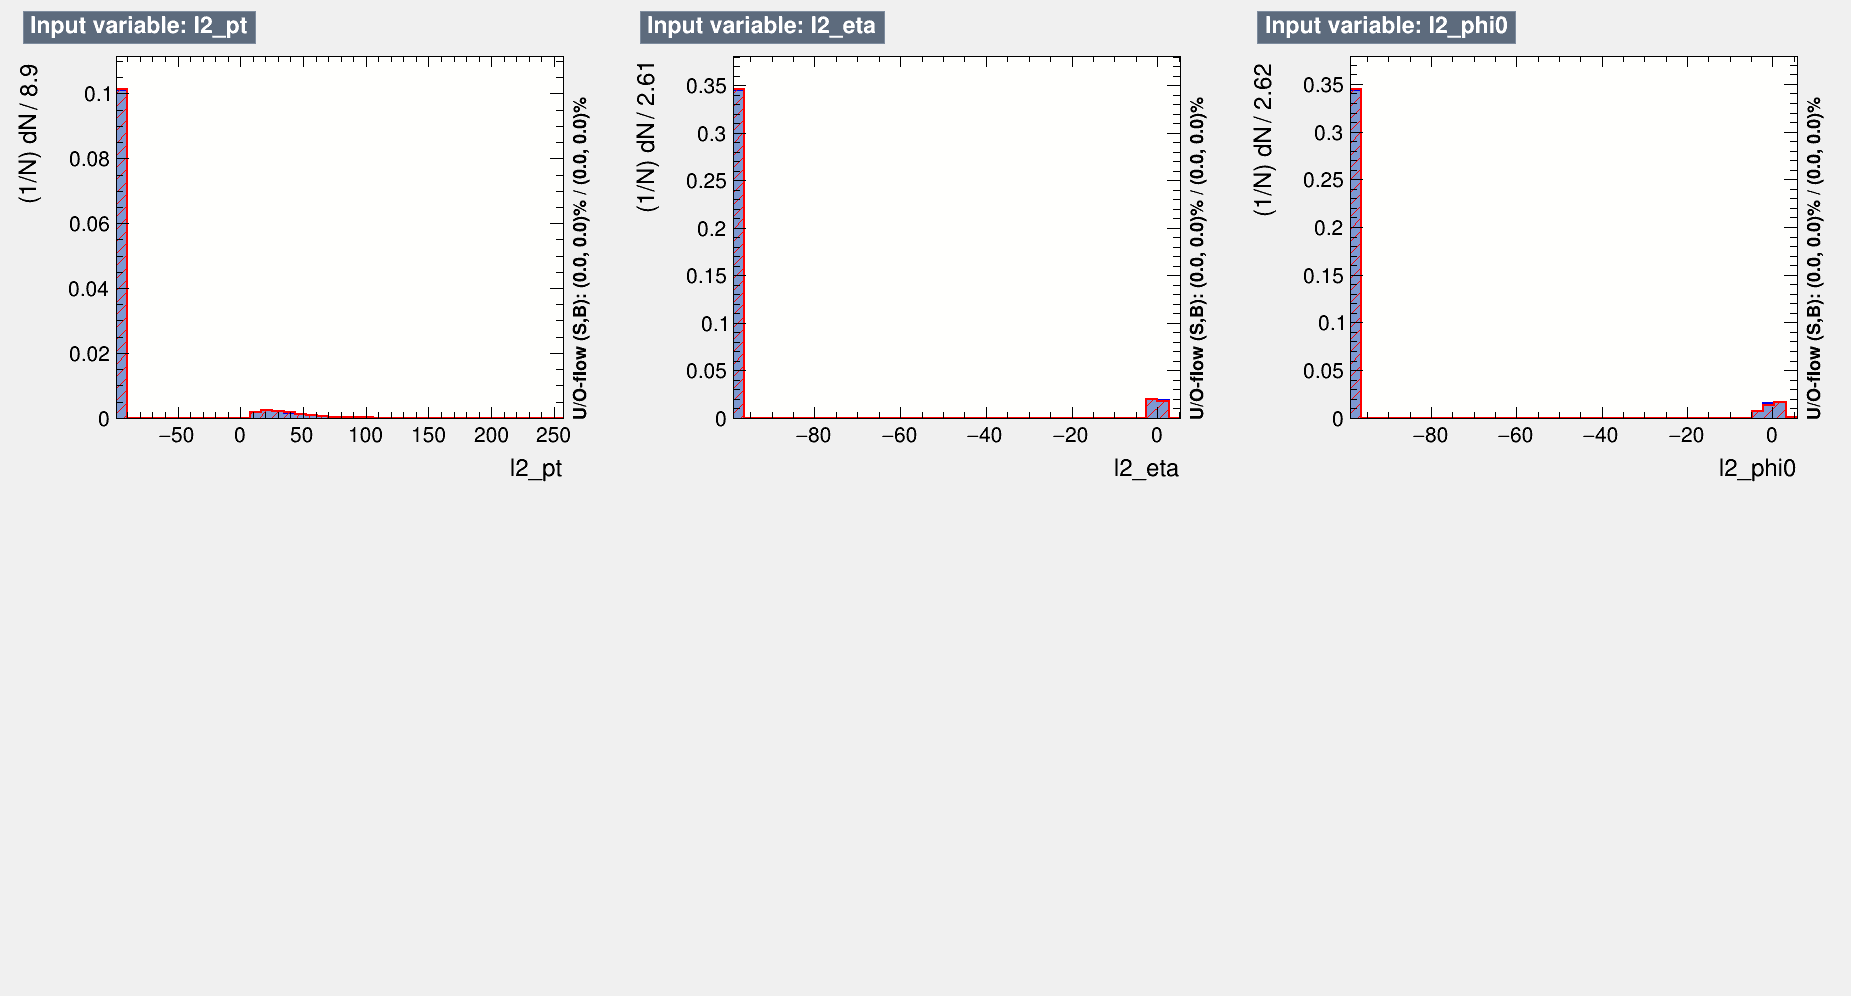
\includegraphics[width=0.62\textwidth]{figures/TMVABDTStudies/lep-vbls4vec/lep4vecvbls6.png}
  \caption{Normalized training variables for the 4-vector BDT, output by TMVA. CP-odd ttH is denoted as "signal" (blue); CP-even ttH is denoted as "background" (red). Variables shown are, from left to right: $p_{T}$ of sub-leading lepton, $\eta$ of sub-leading lepton, and $\phi$ of sub-leading lepton (measured with respect to Higgs candidate).}
  \label{fig:lep4vecvbls6}
\end{figure}

\clearpage

\subsubsection{Results}

We perform a significance comparison between the four-vector and an early iteration of the nominal CP-BDT, recreating the four-vector CP-BDT in xgboost so as to compare both with similar hyperparameter setups. For this study, we use a modified definition of number-counting significance, treating SM $tHjb$ and $tWH$ as background processes and neglecting the modified top Yukawa coupling's effects on $ggH$.

We compare to a Nominal BDT with the following architecture:

In the hadronic channel:

\begin{itemize}
\item $p_{T}$ (scaled by mass) and $\eta$ of the Higgs candidate
\item $p_{T}$, $\eta$, $\phi$ (wrt. Higgs candidate), and BDT score of the first and second reconstructed hadronic tops (see Section \ref{sec:topreco}). In the case where no second top is reconstructed, a missing value is passed to XGBoost.
\item Angles $\Delta\eta$ and $\Delta\phi$ between the top candidates. In the case where no second top is reconstructed, a missing value is passed to XGBoost.
\item Two-object invariant masses $m_{t1H}$, $m_{t2H}$, and $m_{t1t2}$. In the case where no second top is reconstructed, a missing value is passed to XGBoost.
\item Three-object invariant mass $m_{t1t2H}$. In the case where no second top is reconstructed, $m_{t1t2H} = m_{t1H}$.
\item Jet multiplicity and b-jet multiplicity (77\% working point)
\item $H_{T} = \sum_\text{jet j} p^{j}_{T}$
\item $\cos\theta^{*}$
\item Missing $E_{T}$ significance, $E_{T}^\text{miss}/\sqrt{H_{T}}$
\end{itemize}

In the leptonic channel: 

\begin{itemize} 
\item $p_{T}$ (scaled by mass) and $\eta$ of the Higgs candidate
\item $p_{T}$, $\eta$, $\phi$ (wrt. Higgs candidate), and BDT score of the first and second reconstructed hadronic tops (see Section \ref{sec:topreco}). In the case of dilepton events, or if no second top is reconstructed, a missing value is passed to XGBoost.
\item Angles $\Delta\eta$ and $\Delta\phi$ between the top candidates. In the case of dilepton events, or if no second top is reconstructed, a missing value is passed to XGBoost.
\item Two-object invariant masses $m_{t1H}$ $m_{t2H}$, and $m_{t1t2}$. In the case of dilepton events, or if no second top is reconstructed, a missing value is passed to XGBoost.
\item Three-object invariant mass $m_{t1t2H}$. In the case of dilepton events, a missing value is passed to XGBoost. If no second top is reconstructed, $m_{t1t2H} = m_{t1H}$.
\item Jet multiplicity and b-jet multiplicity (77\% working point)
\item $H_{T} = \sum_\text{jet j} p^{j}_{T}$
\item $\cos\theta^{*}$
\item Missing $E_{T}$ significance, $E_{T}^\text{miss}/\sqrt{H_{T}}$
\end{itemize} 

The results of this comparison are shown in Table \ref{tab:appsigs}

\begin{table}[ht]
\begin{center}
\begin{tabular}{lll}
 & Nominal & Alternative \\ \hline
Hadronic ROC AUC & 0.717 & 0.723 \\
Leptonic ROC AUC & 0.708 & 0.718 \\ \hline
$ttH$ significance (if even)& $4.57\sigma$ & $4.60\sigma$ \\
$ttH$ significance (if odd)& $3.26\sigma$ & $3.33\sigma$ \\ \hline
CP odd rejection & $3.01\sigma$ & $2.89\sigma$\\
CP mix rejection & $0.61\sigma$ & $0.59\sigma$ \\ \hline
\hline
\end{tabular}
\end{center}
\vspace{-0.5cm}
\caption{Figures of merit for the fifteen-category CP BDT categorization.  The right-hand column shows that an alternative setup using four-vector training variables in the CP BDT achieves similar sensitivity.}
\label{tab:appsigs}
\end{table}
Ultimately, these results show that, even without the presence of CP-alternative $tH$ samples, the top reconstruction-aided "Nominal" BDT is able to produce a higher Number-Counting Significance than the proposed 4-vector only BDT. As is shown in Figures \ref{fig:nominalBs} - \ref{fig:4vecBs}, the difference is primarily due to the Nominal BDT's ability to reduce $ggH$ contamination by relying on top variables. 

\begin{figure}[htbp]
 \centering
  	\subfloat[Event yield (CP even $ttH$)]{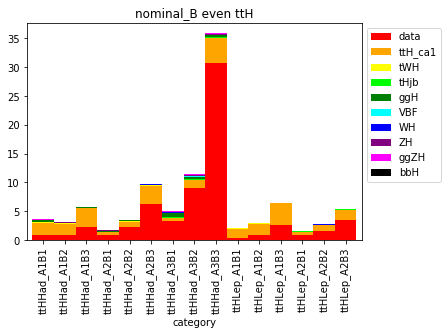
\includegraphics[width=0.42\textwidth]{figures/TMVABDTStudies/nominal_B_e.png}}
	\subfloat[Purity (CP event $ttH$)]{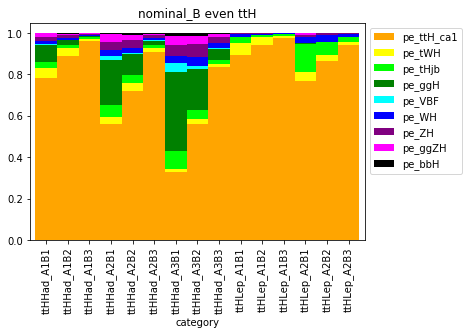
\includegraphics[width=0.42\textwidth]{figures/TMVABDTStudies/nominal_B_pe.png}} \\
  	\subfloat[Event yield (CP odd $ttH$)]{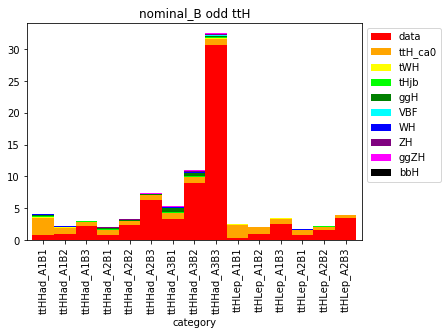
\includegraphics[width=0.42\textwidth]{figures/TMVABDTStudies/nominal_B_o.png}}
	\subfloat[Purity (CP odd $ttH$)]{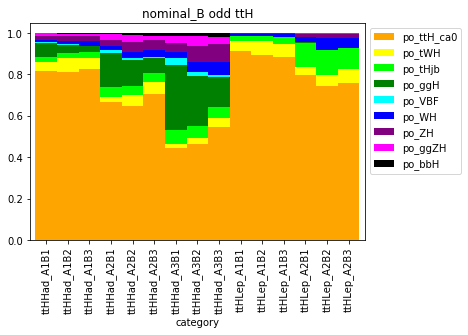
\includegraphics[width=0.42\textwidth]{figures/TMVABDTStudies/nominal_B_po.png}}
  \caption{(Left) Event yields in the CP categories at 139 fb$^{-1}$, with optimized A-boundaries drawn in the BDT score, using the Nominal CP-BDT. Shown separately for CP even $ttH$ (top) and CP odd $ttH$ (bottom). (Right) purity of the Higgs yield in each category for CP even $ttH$ (top) and CP odd $ttH$ (bottom).}
  \label{fig:nominalBs}
\end{figure}

\begin{figure}[htbp]
 \centering
  	\subfloat[Event yield (CP even $ttH$)]{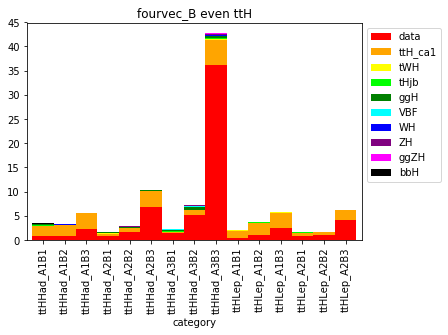
\includegraphics[width=0.42\textwidth]{figures/TMVABDTStudies/4vec_B_e.png}}
	\subfloat[Purity (CP even $ttH$)]{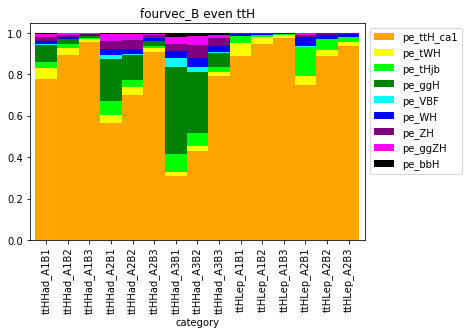
\includegraphics[width=0.42\textwidth]{figures/TMVABDTStudies/4vec_B_pe.png}} \\
  	\subfloat[Event yield (CP odd $ttH$)]{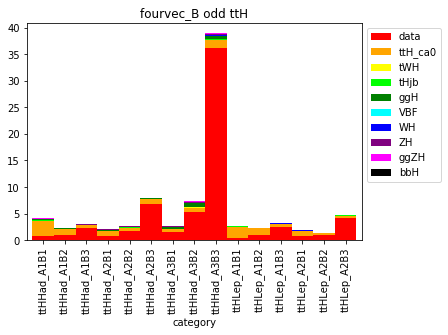
\includegraphics[width=0.42\textwidth]{figures/TMVABDTStudies/4vec_B_o.png}}
	\subfloat[Purity (CP odd $ttH$)]{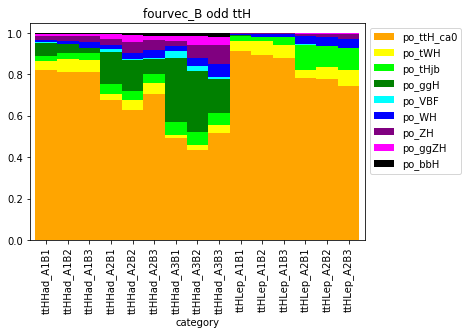
\includegraphics[width=0.42\textwidth]{figures/TMVABDTStudies/4vec_B_po.png}}
  \caption{(Left) Event yields in the CP categories at 139 fb$^{-1}$, with optimized A-boundaries drawn in the BDT score, using the 4-vector CP-BDT. Shown separately for CP even $ttH$ (top) and CP odd $ttH$ (bottom). (Right) purity of the Higgs yield in each category for CP even $ttH$ (top) and CP odd $ttH$ (bottom).}
  \label{fig:4vecBs}
\end{figure}  

\clearpage

\subsection{Dilep/Semilep BDT, ttH Only}

An additional pair of BDTs are developed with the goal of subdividing the leptonic channel into a dedicated semileptonic and dileptonic channel. In order to fully exploit the effectiveness of this technique, a dedicated SBBDT would need to be trained for dileptonic and semileptonic channels as well; however, this is outside the scope of the analysis at this time. Additionally, low event yields in TI sidebands in the dileptonic channel (~8 events passing preselection) call the feasibility of a multi-category fit using this method into question; however, this study may prove useful if this analysis is performed again at the HL-LHC. Dileptonic $ttH$ offers special sensitivity to the top Yukawa coupling due to spin-correlations between the leptonic top decay products, so performing such a category division in the future is well-motivated \cite{Ellis}. 

\subsubsection{Dileptonic BDT}
For the dedicated dileptonic BDT, trained and tested on events which pass the leptonic preselection in addition to requiring that the event contain at least two leptons, we use the following inputs:

\begin{itemize}
\item $p_{T}$, $\eta$, $\phi$, and pseudocontinuous b-tag score of the leading jet in the event
\item $p_{T}$, $\eta$, $\phi$, and pseudocontinuous b-tag score of the leading 2 leptons in the event
\item The $p_{T}$ of the Higgs candidate, scaled by its mass
\item  $\cos$($\theta^{*}$)
\item The $p_{T}$ and $\eta$ of the two leading photons in the event
\item The magnitude and $\phi$ of the missing transverse energy in the event
\item The summed invariant mass of all jets in the event
\item The minimum $\Delta$R between a photon and a jet in the event
\item The $\Delta$R between the two leptons in the event
\end{itemize} 

The linear correlations between these variables in $ttH$ CP even and CP odd aMCnlo+Pythia8 Monte Carlo are shown in Figure \ref{fig:dilepcorr4vec}.  Figures \ref{fig:dilep4vecvbls1} - \ref{fig:dilep4vecvbls4} compare the distribution of each training variable in $ttH$ CP even and CP odd Monte Carlo. We report a ROC-AUC of 0.707 for this BDT.

\begin{figure}[htbp]
  \centering
    \subfloat[CP Even $ttH$]{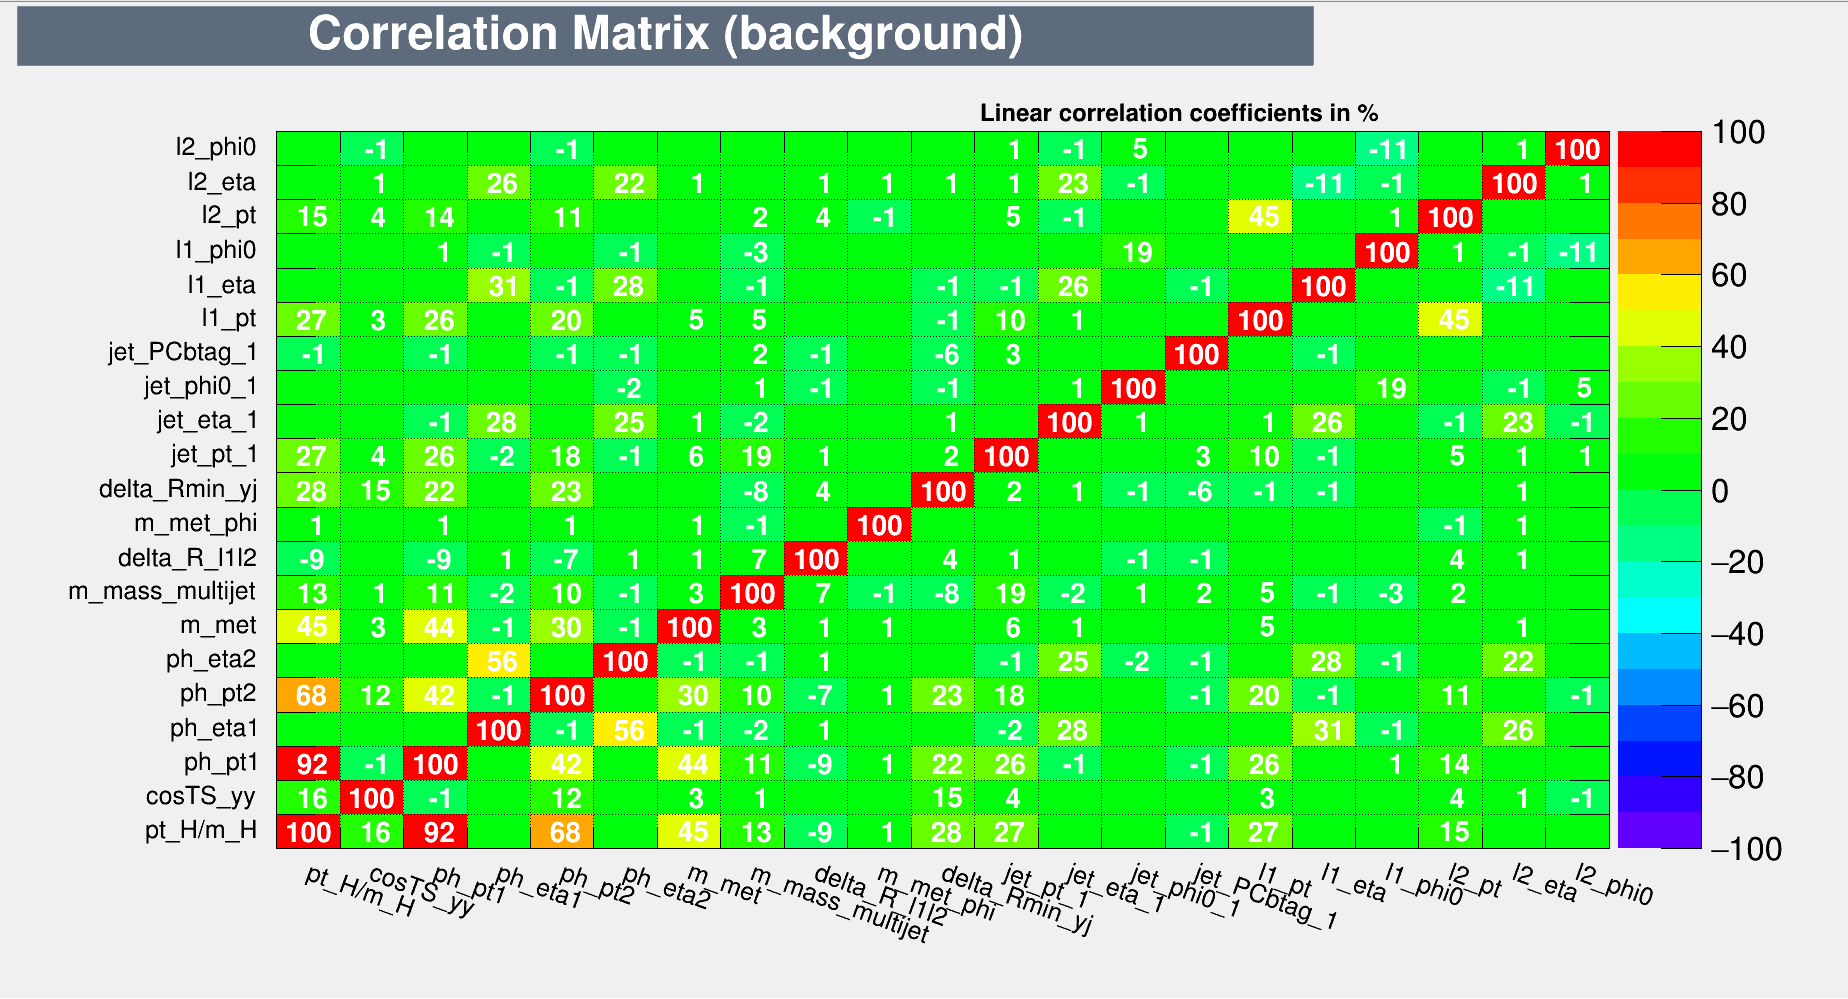
\includegraphics[width=0.62\textwidth]{figures/TMVABDTStudies/dilep-vbls4vec/dilep4veccorrMatEven.png}}\\
	\subfloat[CP Odd $ttH$]{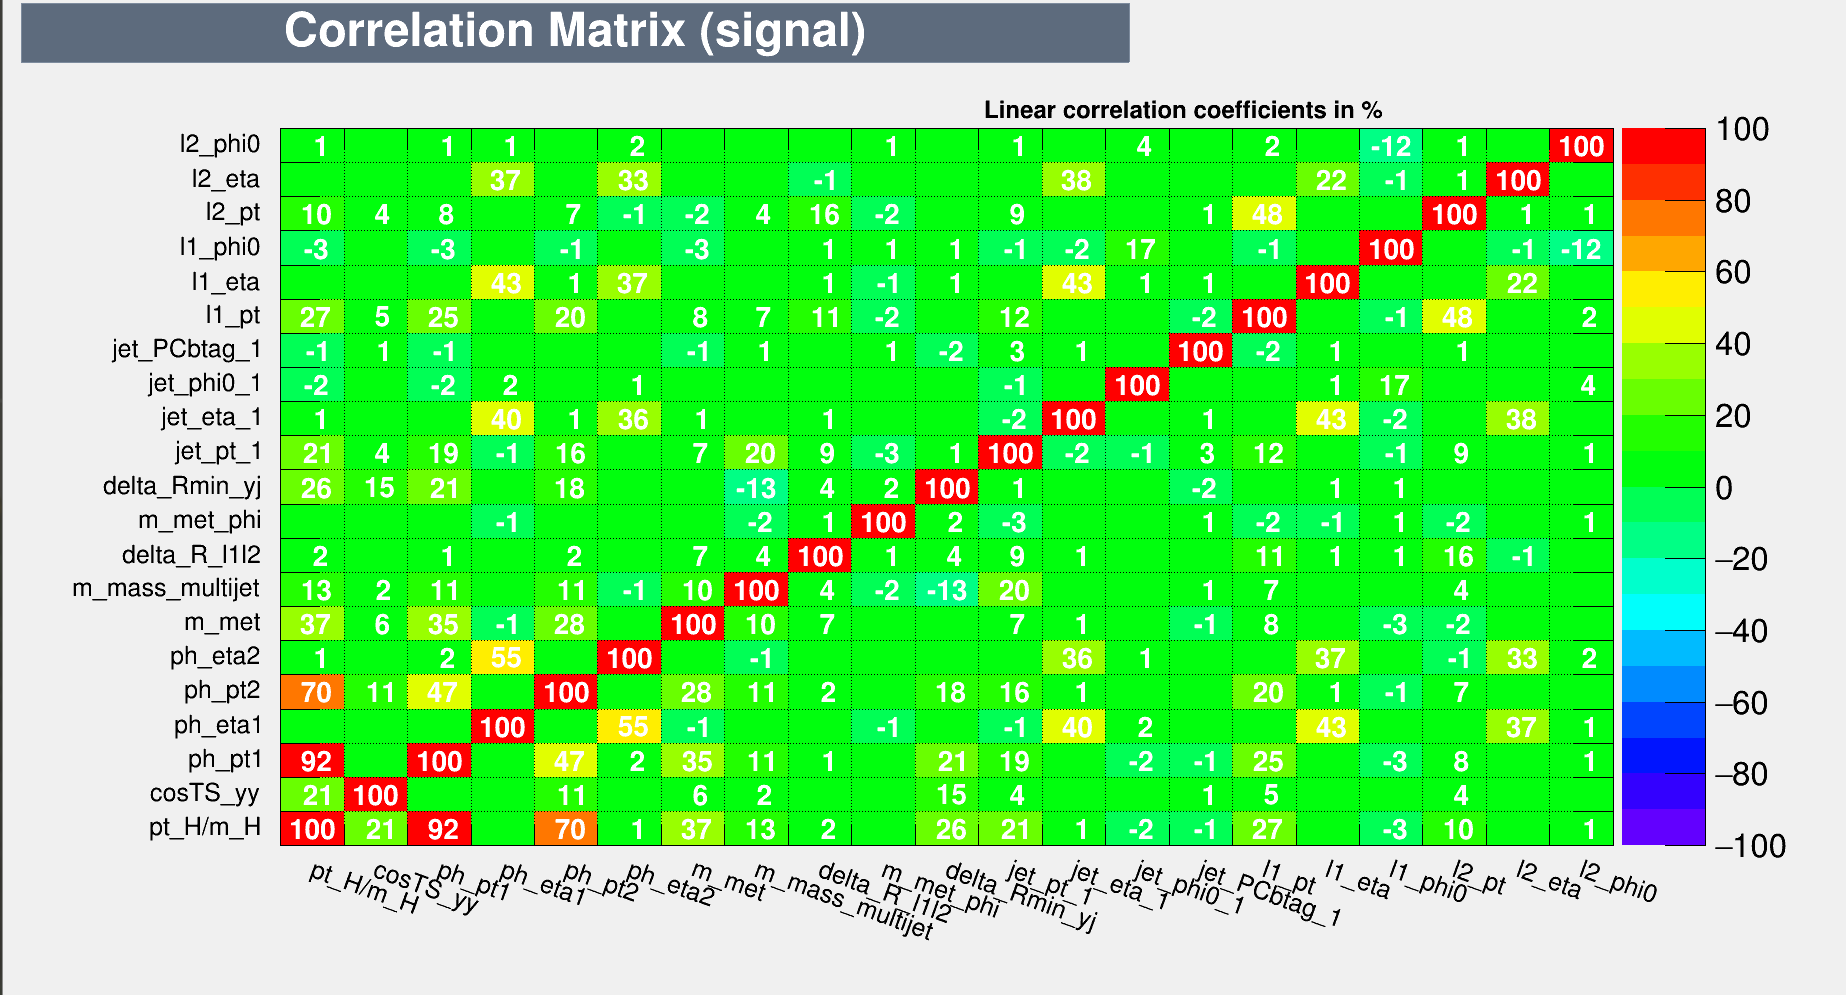
\includegraphics[width=0.62\textwidth]{figures/TMVABDTStudies/dilep-vbls4vec/dilep4veccorrMatOdd.png}} 
 \caption{Training variable correlations for events passing dileptonic pre-selection.}
  \label{fig:dilepcorr4vec}
\end{figure}
\begin{figure}[htbp]
  \centering
  	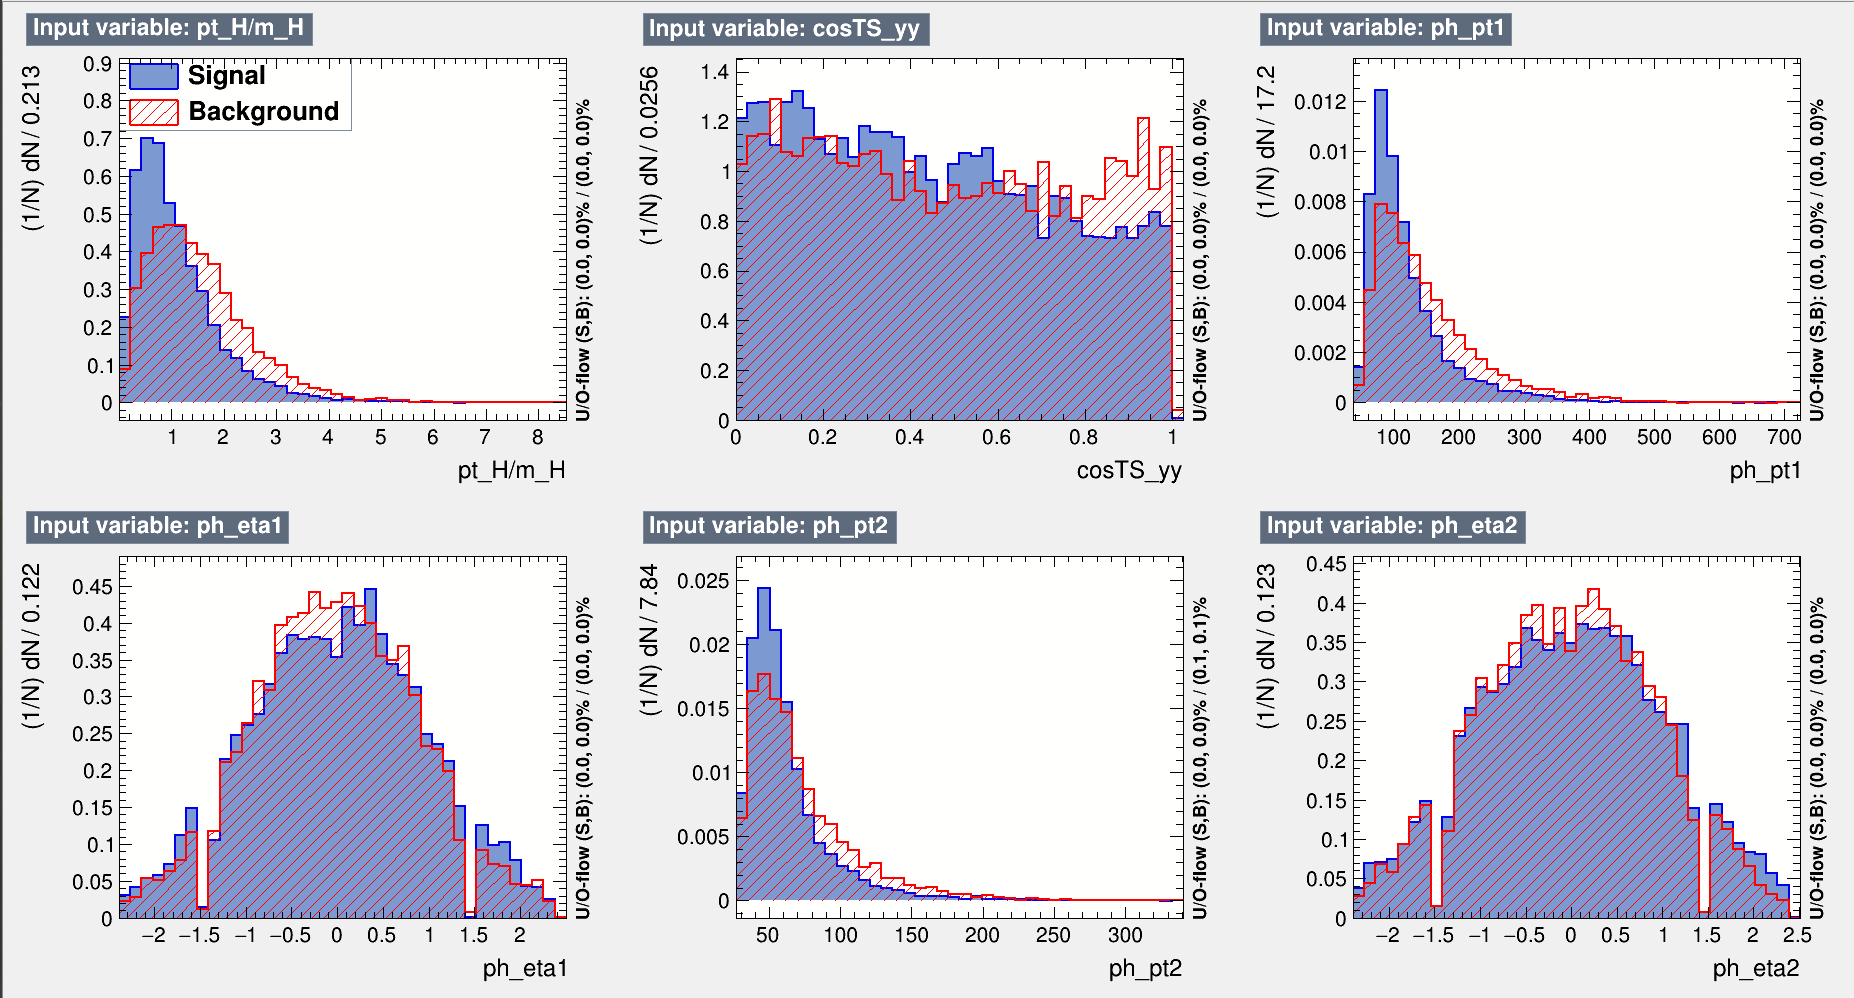
\includegraphics[width=0.62\textwidth]{figures/TMVABDTStudies/dilep-vbls4vec/dilep4vecvbls1.png}
  \caption{Normalized training variables for the 4-vector BDT, output by TMVA. CP-odd ttH is denoted as "signal" (blue); CP-even ttH is denoted as "background" (red). Variables shown are, from left to right, top row to bottom row: Higgs candidate $p_{T}$ (scaled by mass), $\cos$($\theta^{*}$), leading photon $p_{T}$, leading photon $\eta$, subleading photon $p_{T}$, subleading photon $\eta$.}
  \label{fig:dilep4vecvbls1}
\end{figure}

\begin{figure}[htbp]
  \centering
  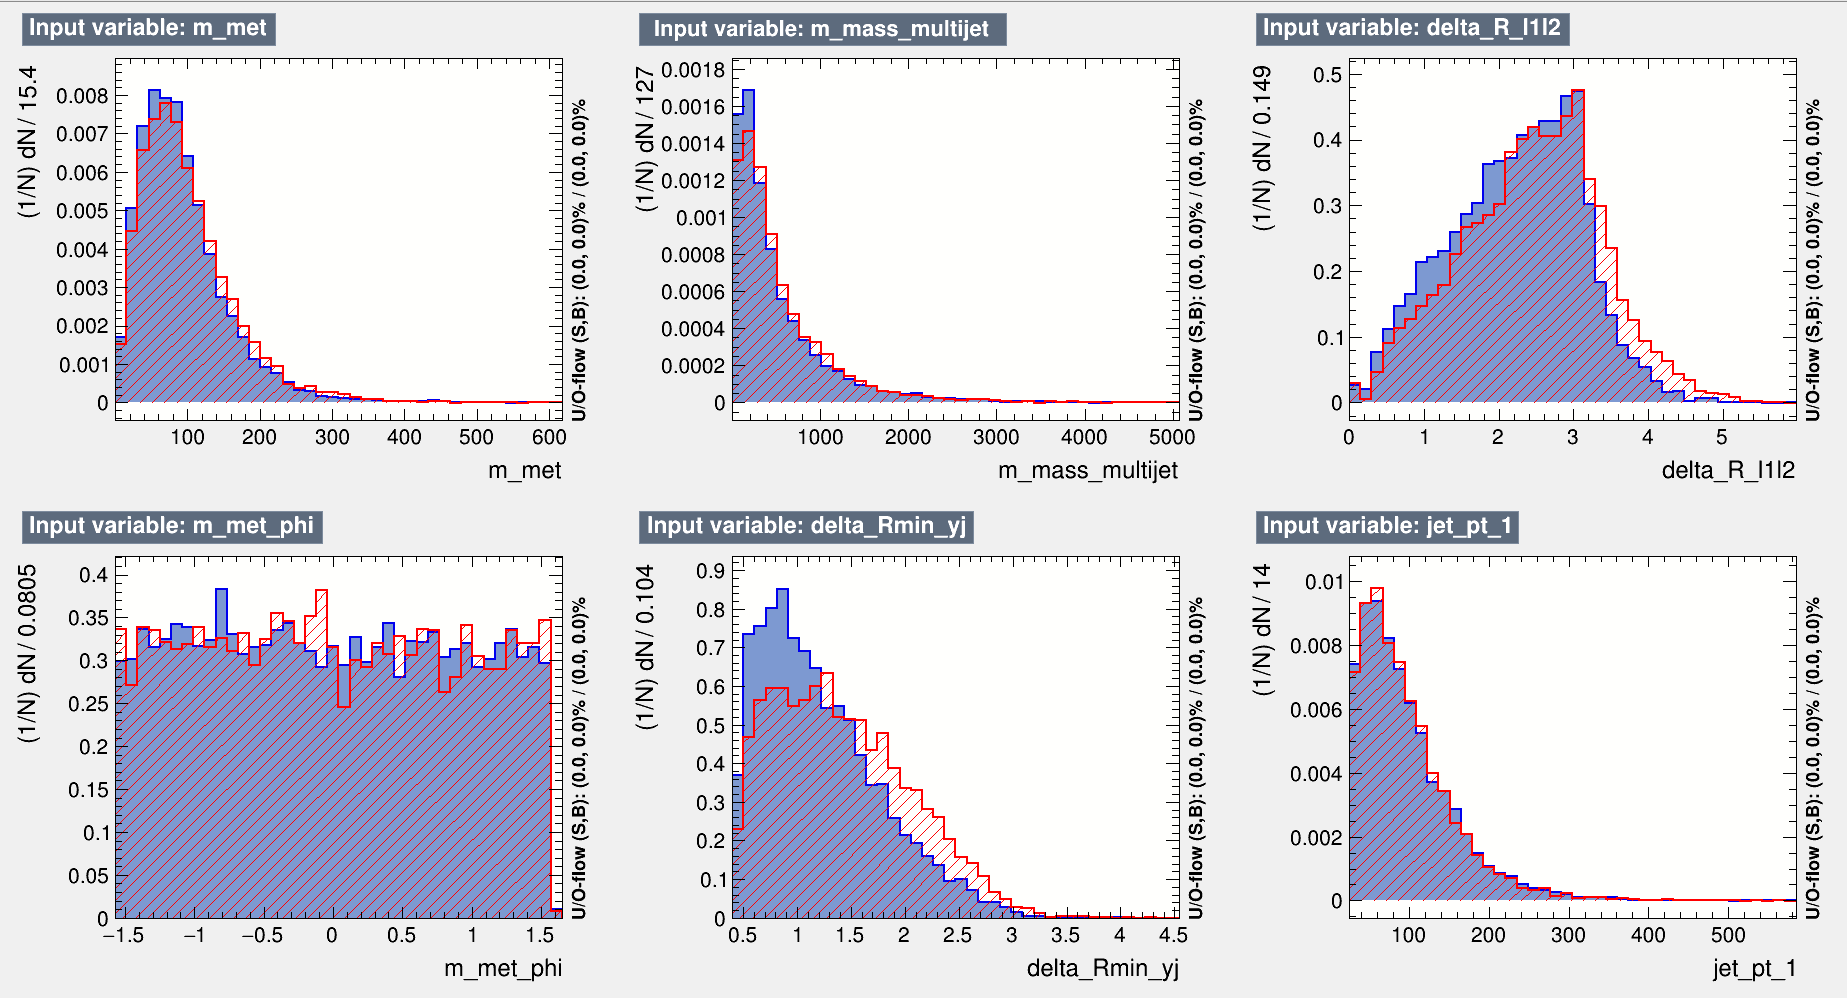
\includegraphics[width=0.62\textwidth]{figures/TMVABDTStudies/dilep-vbls4vec/dilep4vecvbls2.png}
  \caption{Normalized training variables for the 4-vector BDT, output by TMVA. CP-odd ttH is denoted as "signal" (blue); CP-even ttH is denoted as "background" (red). Variables shown are, from left to right, top row to bottom row: Magnitude of MET, summed invariant mass of all jets in the event, $\Delta$R between the two leptons present in the event, MET $\phi$ (branch cut chosen to range from -$\pi$/2 to $\pi$/2), minimum $\Delta$R between a photon and a jet, $p_{T}$ of highest b-tag scoring jet}
  \label{fig:dilep4vecvbls2}
\end{figure}

\begin{figure}[htbp]
  \centering
  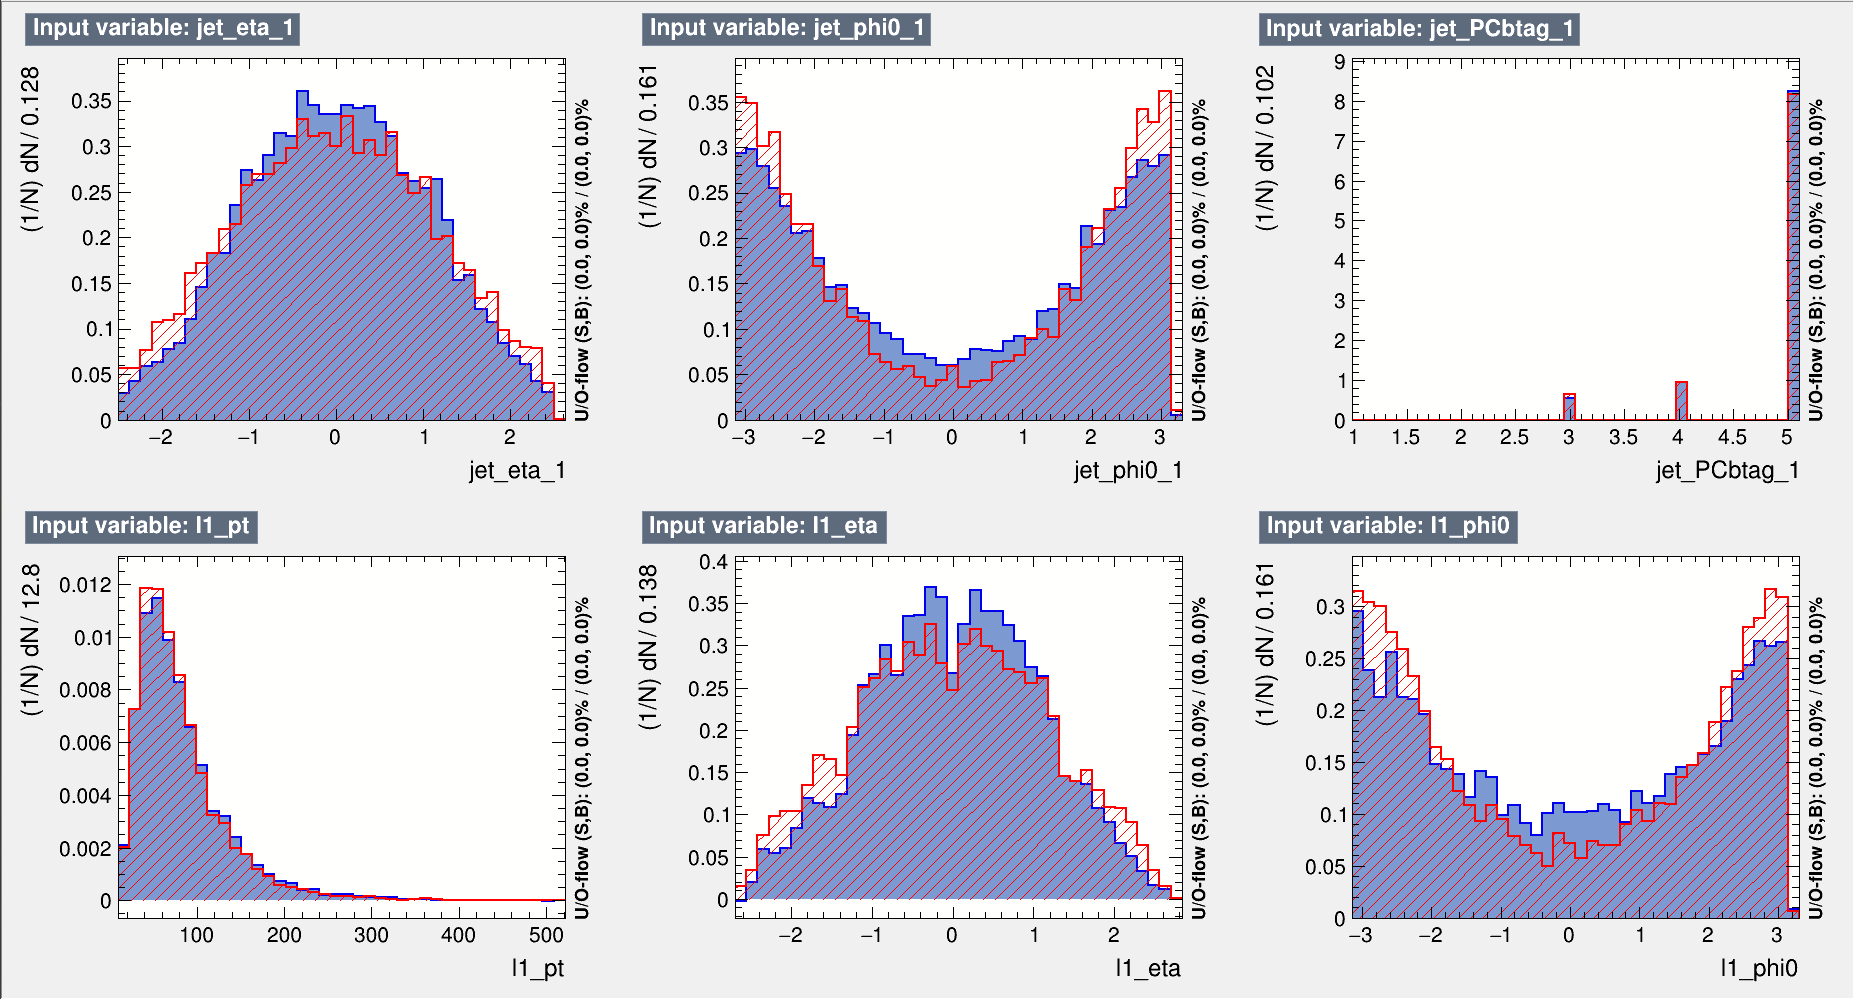
\includegraphics[width=0.62\textwidth]{figures/TMVABDTStudies/dilep-vbls4vec/dilep4vecvbls3.png}
  \caption{Normalized training variables for the 4-vector BDT, output by TMVA. CP-odd ttH is denoted as "signal" (blue); CP-even ttH is denoted as "background" (red). Variables shown are, from left to right, top row to bottom row: $\eta$ of highest b-tag scoring jet, $\phi$ of highest btag-scoring jet (measured with respect to the Higgs candidate), pseudo-continuous b-tag score of highest btag-scoring jet,  $p_{T}$ of leading lepton, $\eta$ of leading lepton, $\phi$ of leading lepton (measured with respect to the Higgs candidate)}
  \label{fig:dilep4vecvbls3}
\end{figure}

\begin{figure}[htbp]
  \centering
  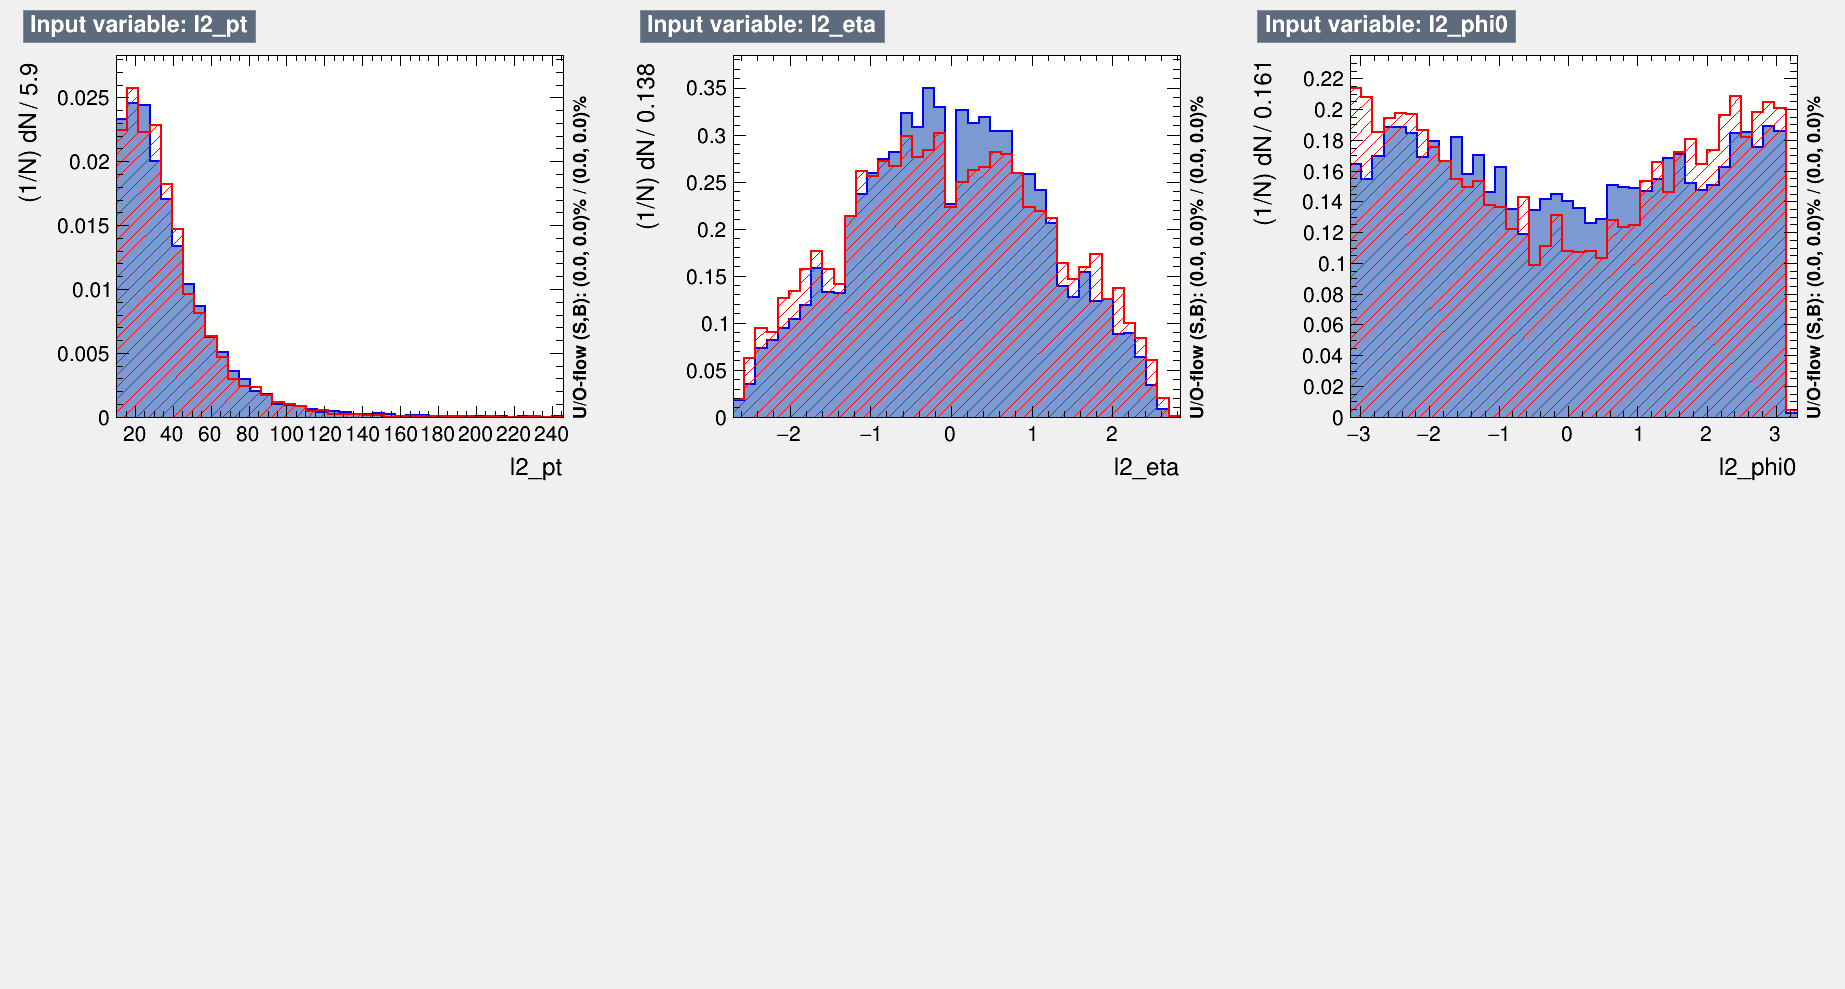
\includegraphics[width=0.62\textwidth]{figures/TMVABDTStudies/dilep-vbls4vec/dilep4vecvbls4.png}
  \caption{Normalized training variables for the 4-vector BDT, output by TMVA. CP-odd ttH is denoted as "signal" (blue); CP-even ttH is denoted as "background" (red). Variables shown are, from left to right, top row to bottom row: $p_{T}$ of subleading lepton, $\eta$ of subleading lepton, $\phi$ of subleading lepton (measured with respect to the Higgs candidate)}
  \label{fig:dilep4vecvbls4}
\end{figure}

\subsubsection{Semileptonic BDT}
For the dedicated semileptonic BDT, trained and tested on events which pass the leptonic preselection in addition to requiring that the event contain exactly one lepton, we use the following inputs:
\begin{itemize}
\item $p_{T}$, $\eta$, $\phi$, and pseudocontinuous b-tag score of the leading 4 jets in the event
\item $p_{T}$, $\eta$, $\phi$, and pseudocontinuous b-tag score of the leading lepton in the event
\item The $p_{T}$ of the Higgs candidate (scaled by mass)
\item  $\cos$($\theta^{*}$)
\item The $\eta$ and $\phi$ of the two leading photons in the event
\item The magnitude and $\phi$ of the missing transverse energy in the event
\end{itemize} 

The linear correlations between these variables in $ttH$ CP even and CP odd aMCnlo+Pythia8 Monte Carlo are shown in Figure \ref{fig:semilepcorr4vec}.  Figures \ref{fig:semilep4vecvbls1} - \ref{fig:semilep4vecvbls5} compare the distribution of each training variable in $ttH$ CP even and CP odd Monte Carlo. We report a ROC-AUC of 0.725 for this BDT.

\begin{figure}[htbp]
  \centering
  	\subfloat[CP Even $ttH$]{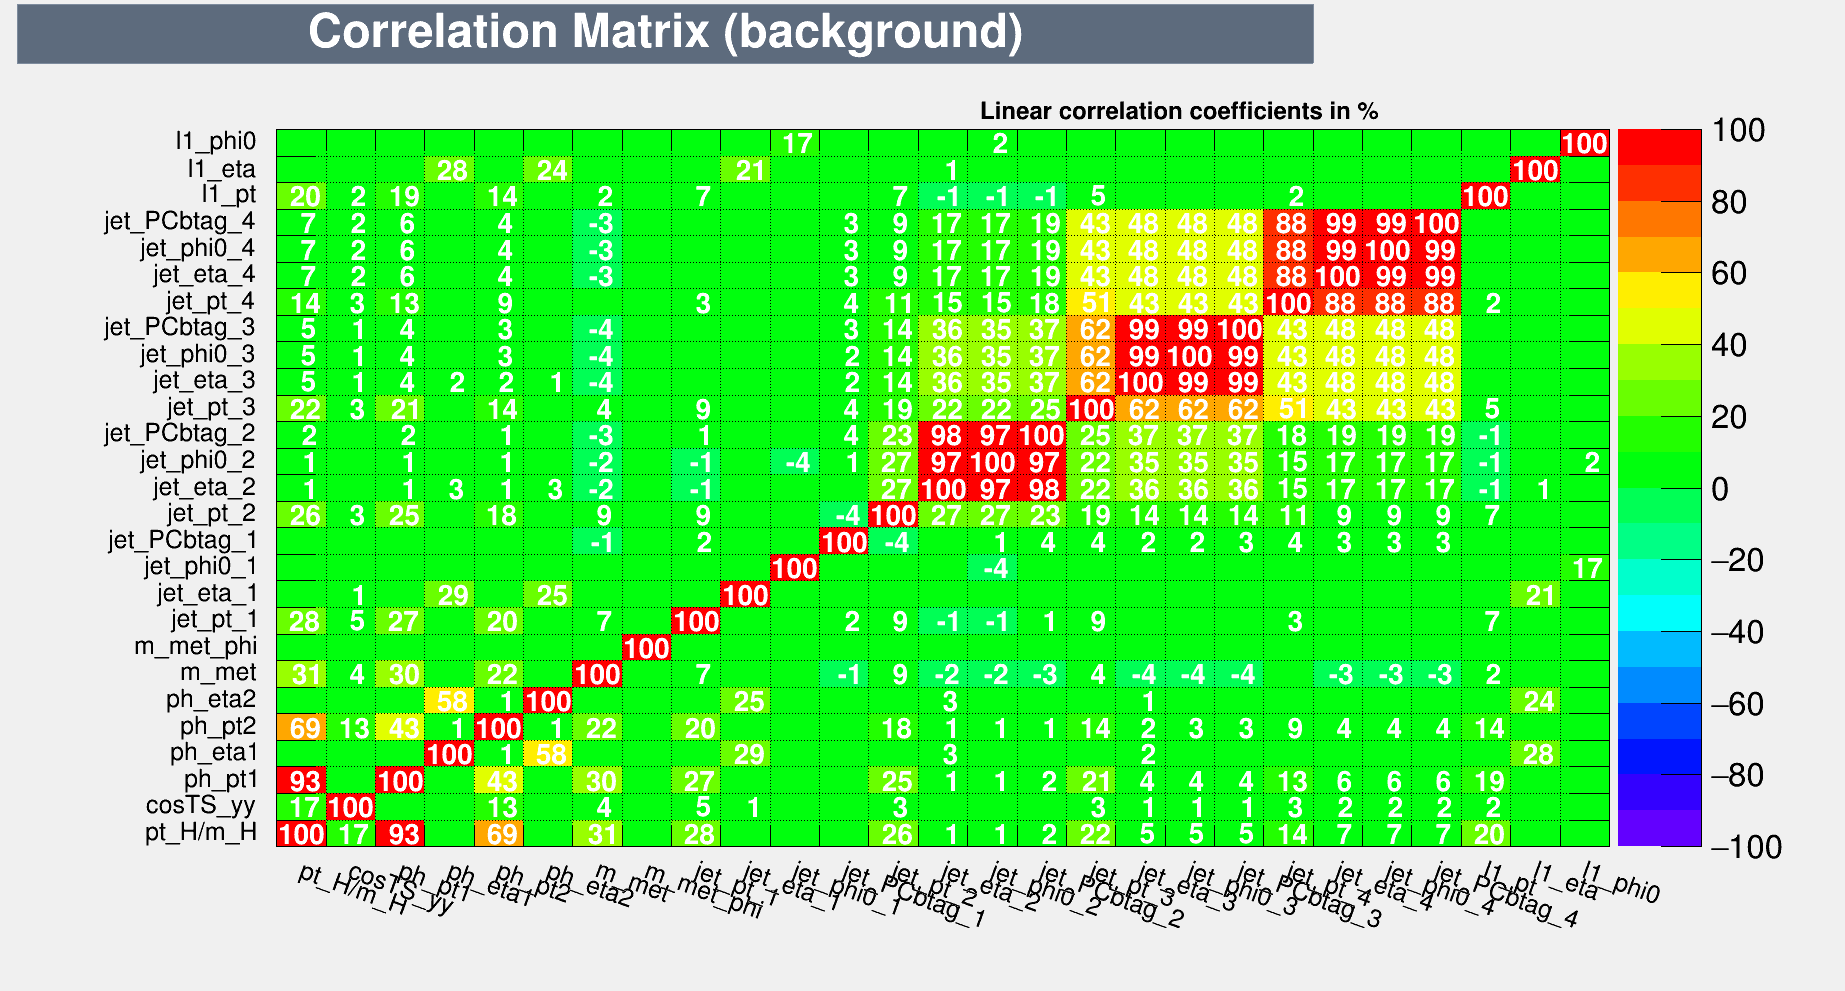
\includegraphics[width=0.62\textwidth]{figures/TMVABDTStudies/semilep-vbls4vec/semilep4veccorrMatEven.png}}\\
	\subfloat[CP Odd $ttH$]{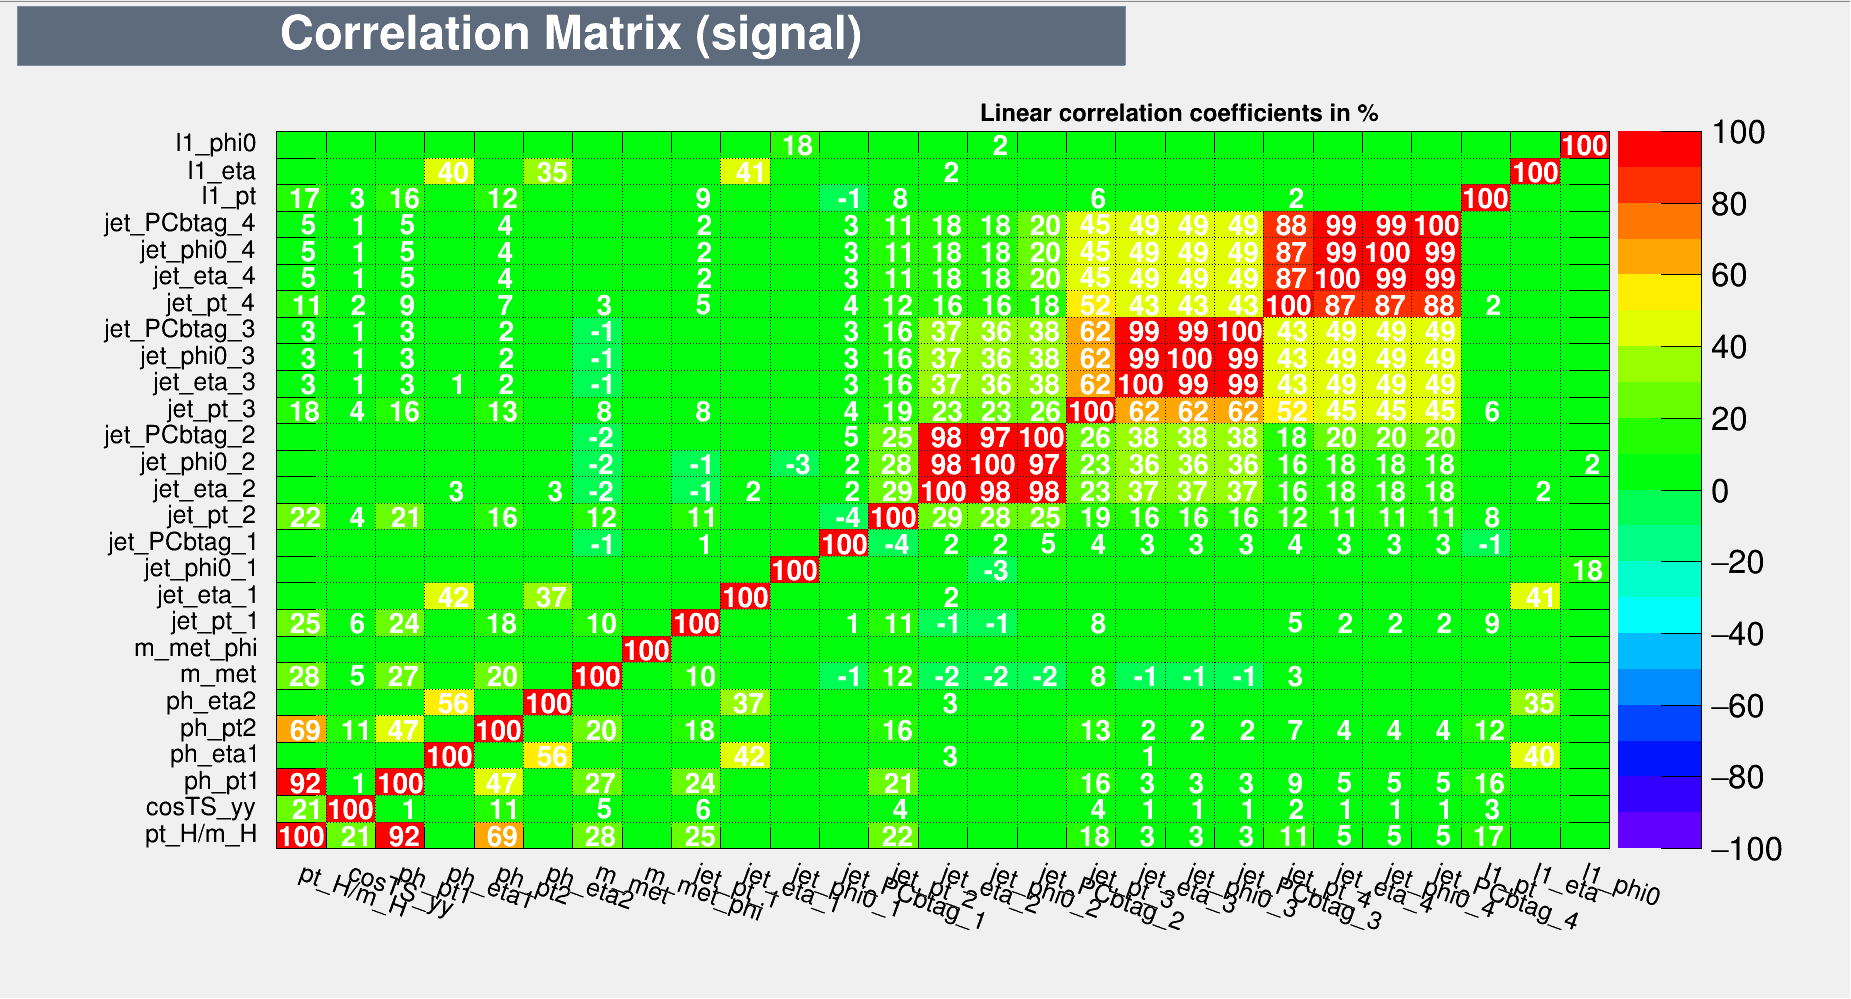
\includegraphics[width=0.62\textwidth]{figures/TMVABDTStudies/semilep-vbls4vec/semilep4veccorrMatOdd.png}} 
 \caption{Training variable correlations for events passing semileptonic pre-selection.}
 \label{fig:semilepcorr4vec}
  
\end{figure}
\begin{figure}[htbp]
  \centering
  	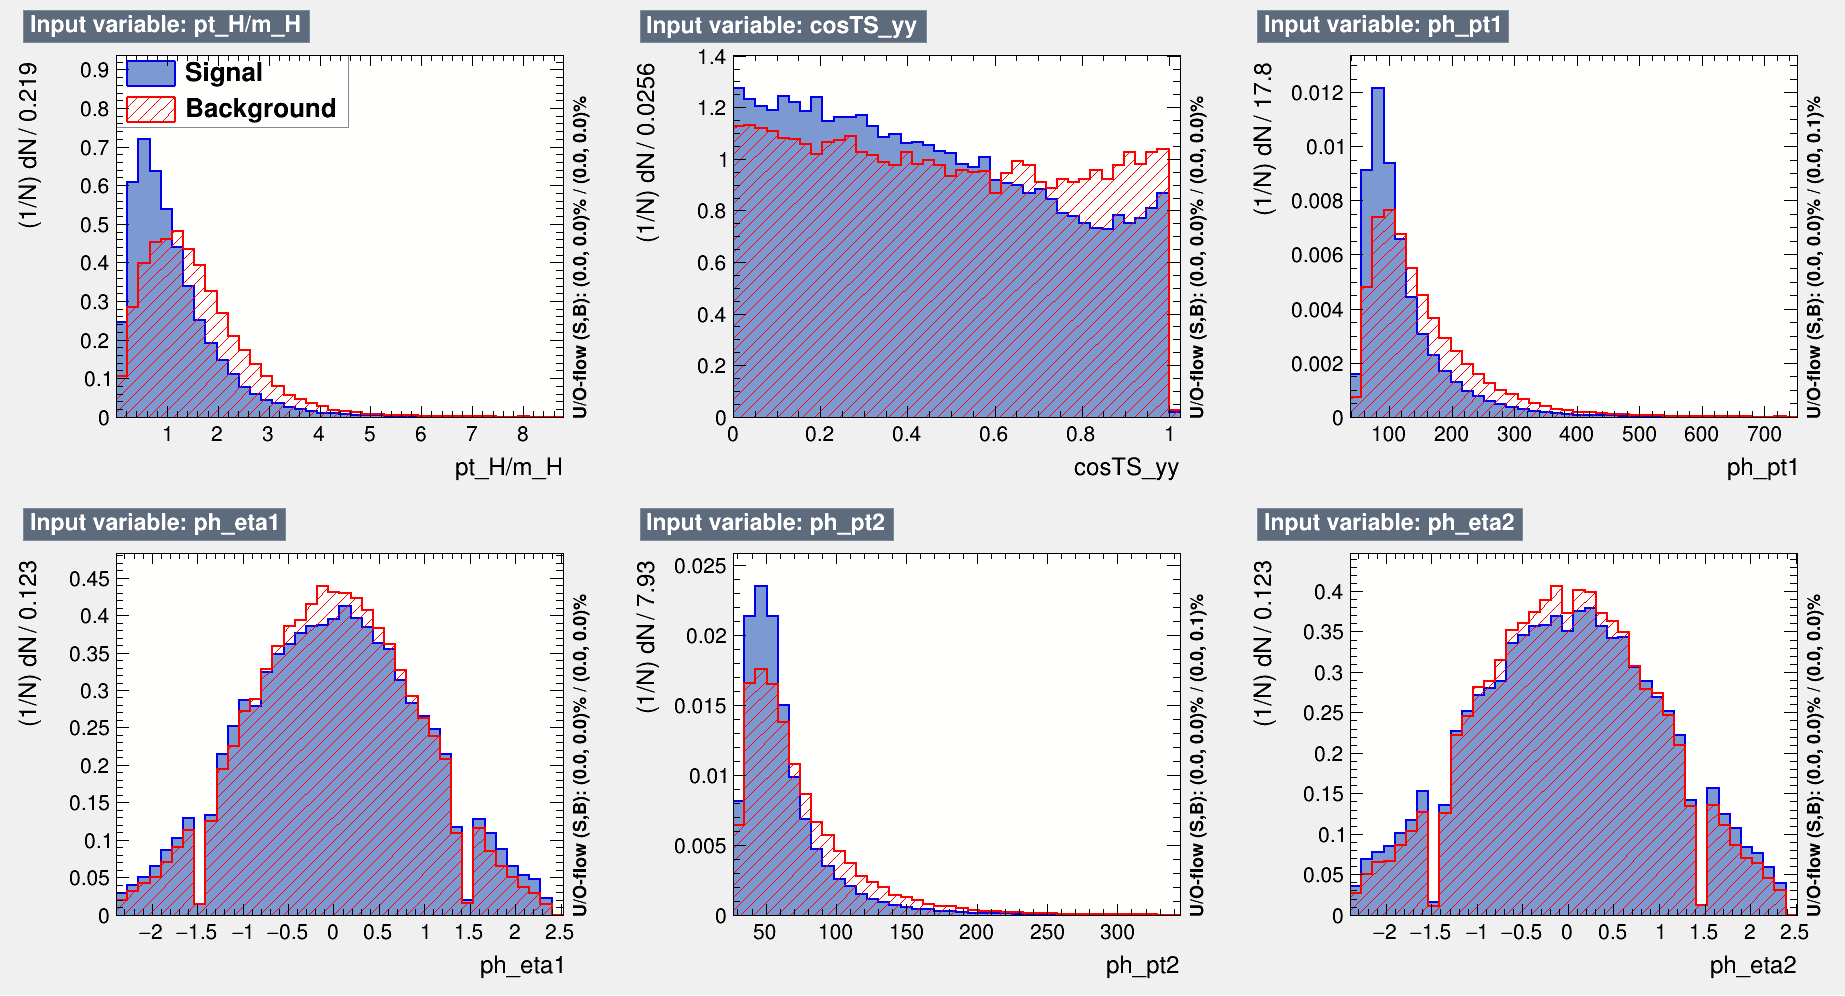
\includegraphics[width=0.62\textwidth]{figures/TMVABDTStudies/semilep-vbls4vec/semilep4vecvbls1.png}
    \caption{Normalized training variables for the 4-vector BDT, output by TMVA. CP-odd ttH is denoted as "signal" (blue); CP-even ttH is denoted as "background" (red). Variables shown are, from left to right, top row to bottom row: Higgs candidate $p_{T}$ (scaled by mass), $\cos$($\theta^{*}$), leading photon $p_{T}$, leading photon $\eta$, subleading photon $p_{T}$, subleading photon $\eta$.}
  \label{fig:semilep4vecvbls1}
\end{figure}

\begin{figure}[htbp]
  \centering
  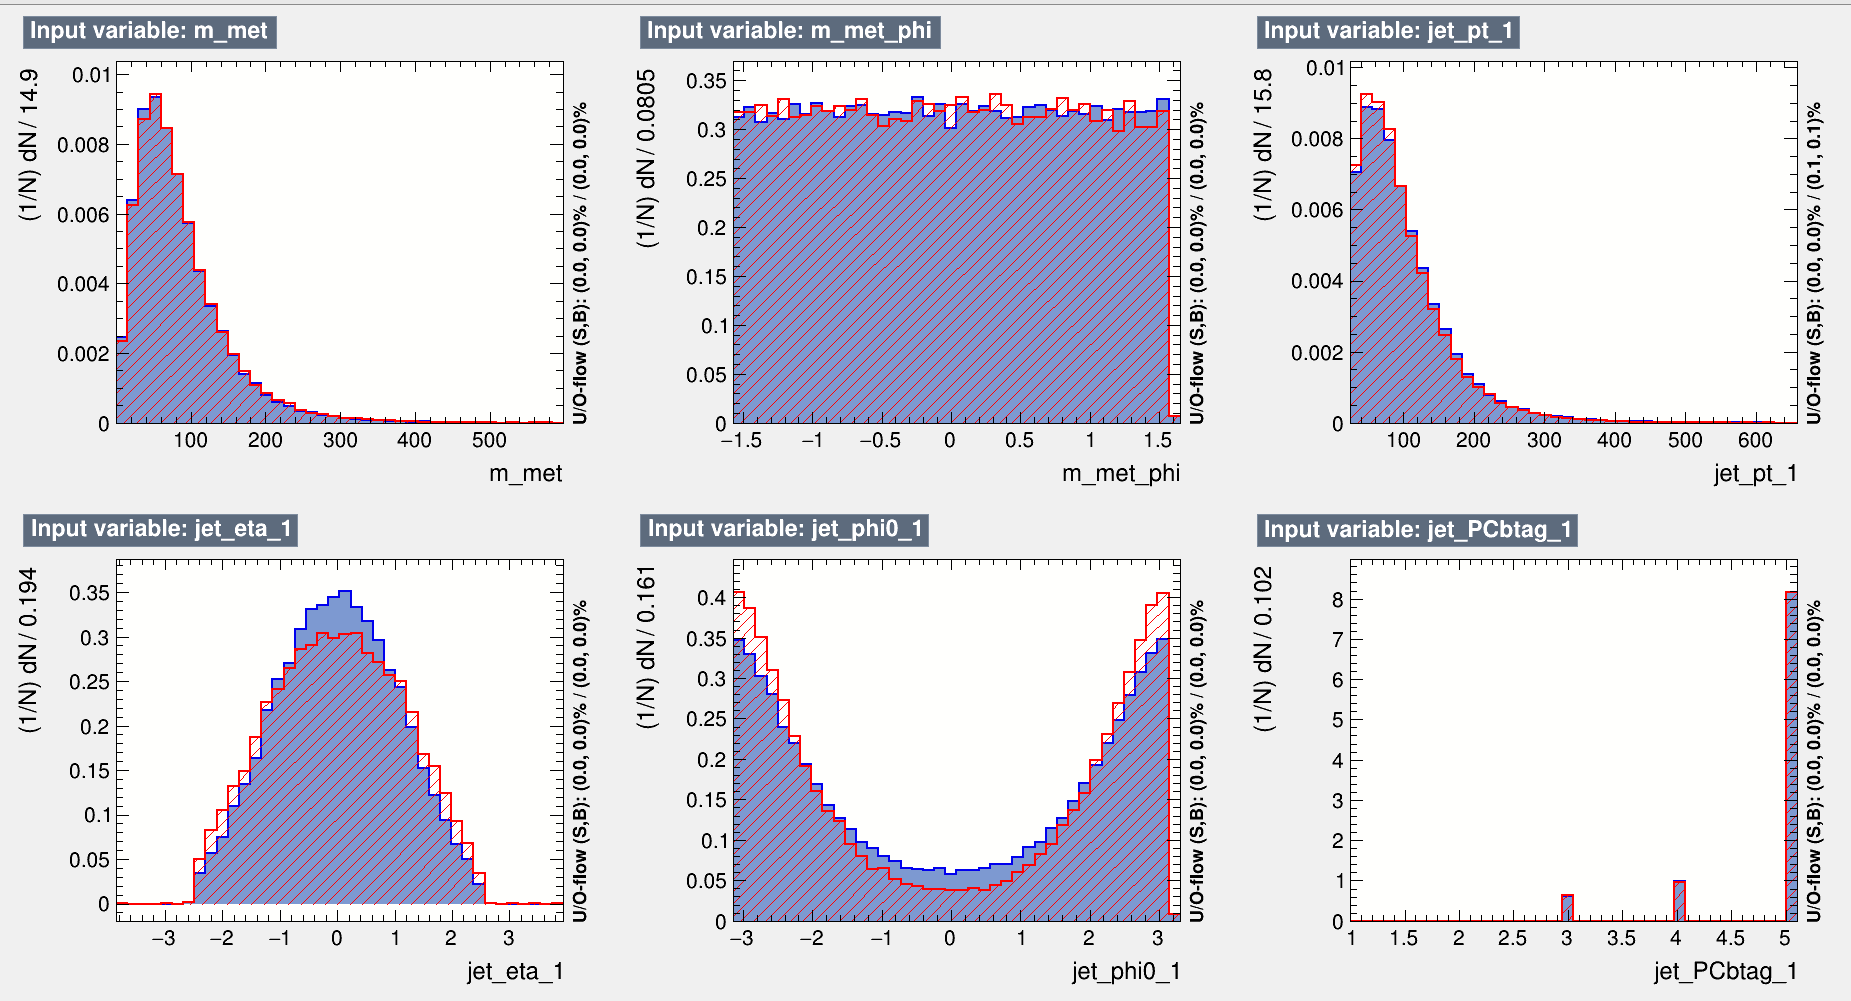
\includegraphics[width=0.62\textwidth]{figures/TMVABDTStudies/semilep-vbls4vec/semilep4vecvbls2.png}
  \caption{Normalized training variables for the 4-vector BDT, output by TMVA. CP-odd ttH is denoted as "signal" (blue); CP-even ttH is denoted as "background" (red). Variables shown are, from left to right, top row to bottom row: Magnitude of the event MET, MET $\phi$ (branch cut chosen to range from -$\pi$/2 to $\pi$/2), $p_{T}$ of highest b-tag scoring jet, $\eta$ of highest b-tag scoring jet, $\phi$ of highest btag-scoring jet (measured with respect to the Higgs candidate), pseudo-continuous b-tag score of highest btag-scoring jet}
  \label{fig:semilep4vecvbls2}
\end{figure}

\begin{figure}[htbp]
  \centering
  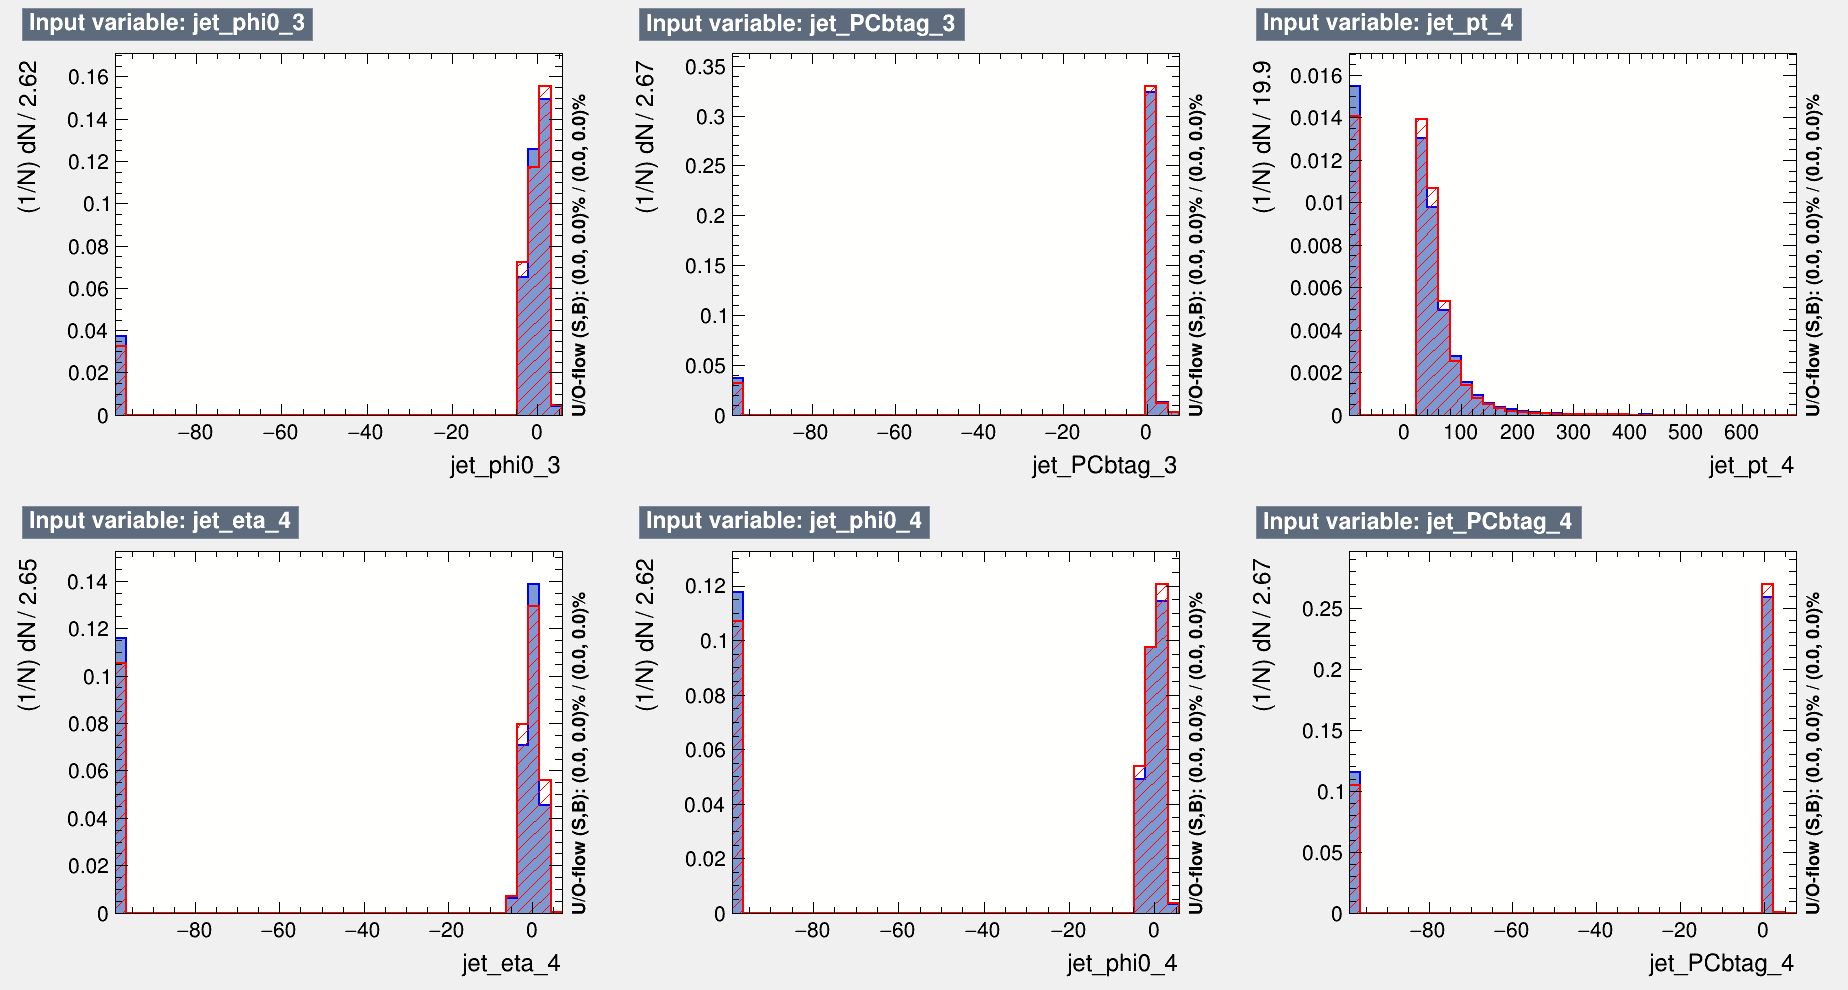
\includegraphics[width=0.62\textwidth]{figures/TMVABDTStudies/semilep-vbls4vec/semilep4vecvbls4.png}
  \caption{Normalized training variables for the 4-vector BDT, output by TMVA. CP-odd ttH is denoted as "signal" (blue); CP-even ttH is denoted as "background" (red). Variables shown are, from left to right, top row to bottom row: $p_{T}$ of second-highest b-tag scoring jet, $\eta$ of second-highest b-tag scoring jet, $\phi$ of second-highest btag-scoring jet (measured with respect to the Higgs candidate), pseudo-continuous b-tag score of second-highest btag-scoring jet, $p_{T}$ of third-highest b-tag scoring jet, $\eta$ of third-highest b-tag scoring jet}
  \label{fig:semilep4vecvbls4}
\end{figure}

\begin{figure}[htbp]
  \centering
  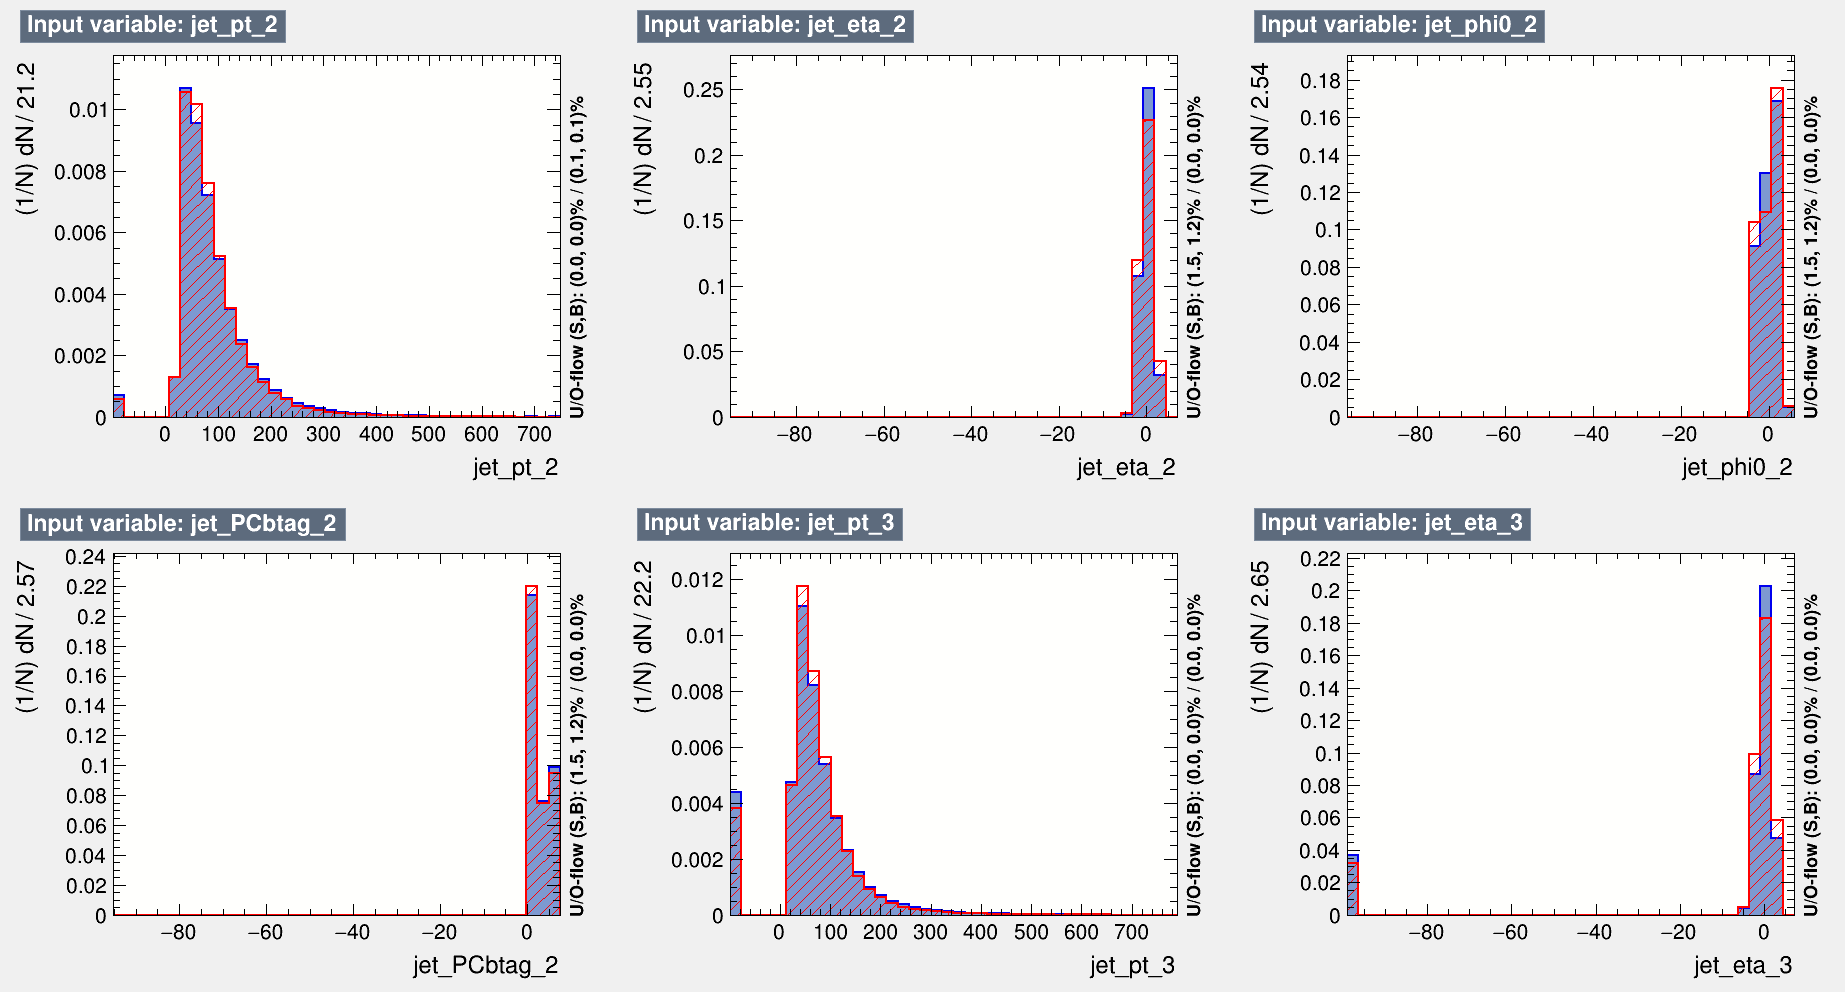
\includegraphics[width=0.62\textwidth]{figures/TMVABDTStudies/semilep-vbls4vec/semilep4vecvbls3.png}
  \caption{Normalized training variables for the 4-vector BDT, output by TMVA. CP-odd ttH is denoted as "signal" (blue); CP-even ttH is denoted as "background" (red). Variables shown are, from left to right, top row to bottom row: $\phi$ of third-highest btag-scoring jet (measured with respect to the Higgs candidate), pseudo-continuous b-tag score of third-highest btag-scoring jet, $p_{T}$ of fourth-highest b-tag scoring jet, $\eta$ of fourth-highest b-tag scoring jet, $\phi$ of fourth-highest btag-scoring jet (measured with respect to the Higgs candidate), pseudo-continuous b-tag score of fourth-highest btag-scoring jet}
  \label{fig:semilep4vecvbls3}
\end{figure}


\begin{figure}[htbp]
  \centering
  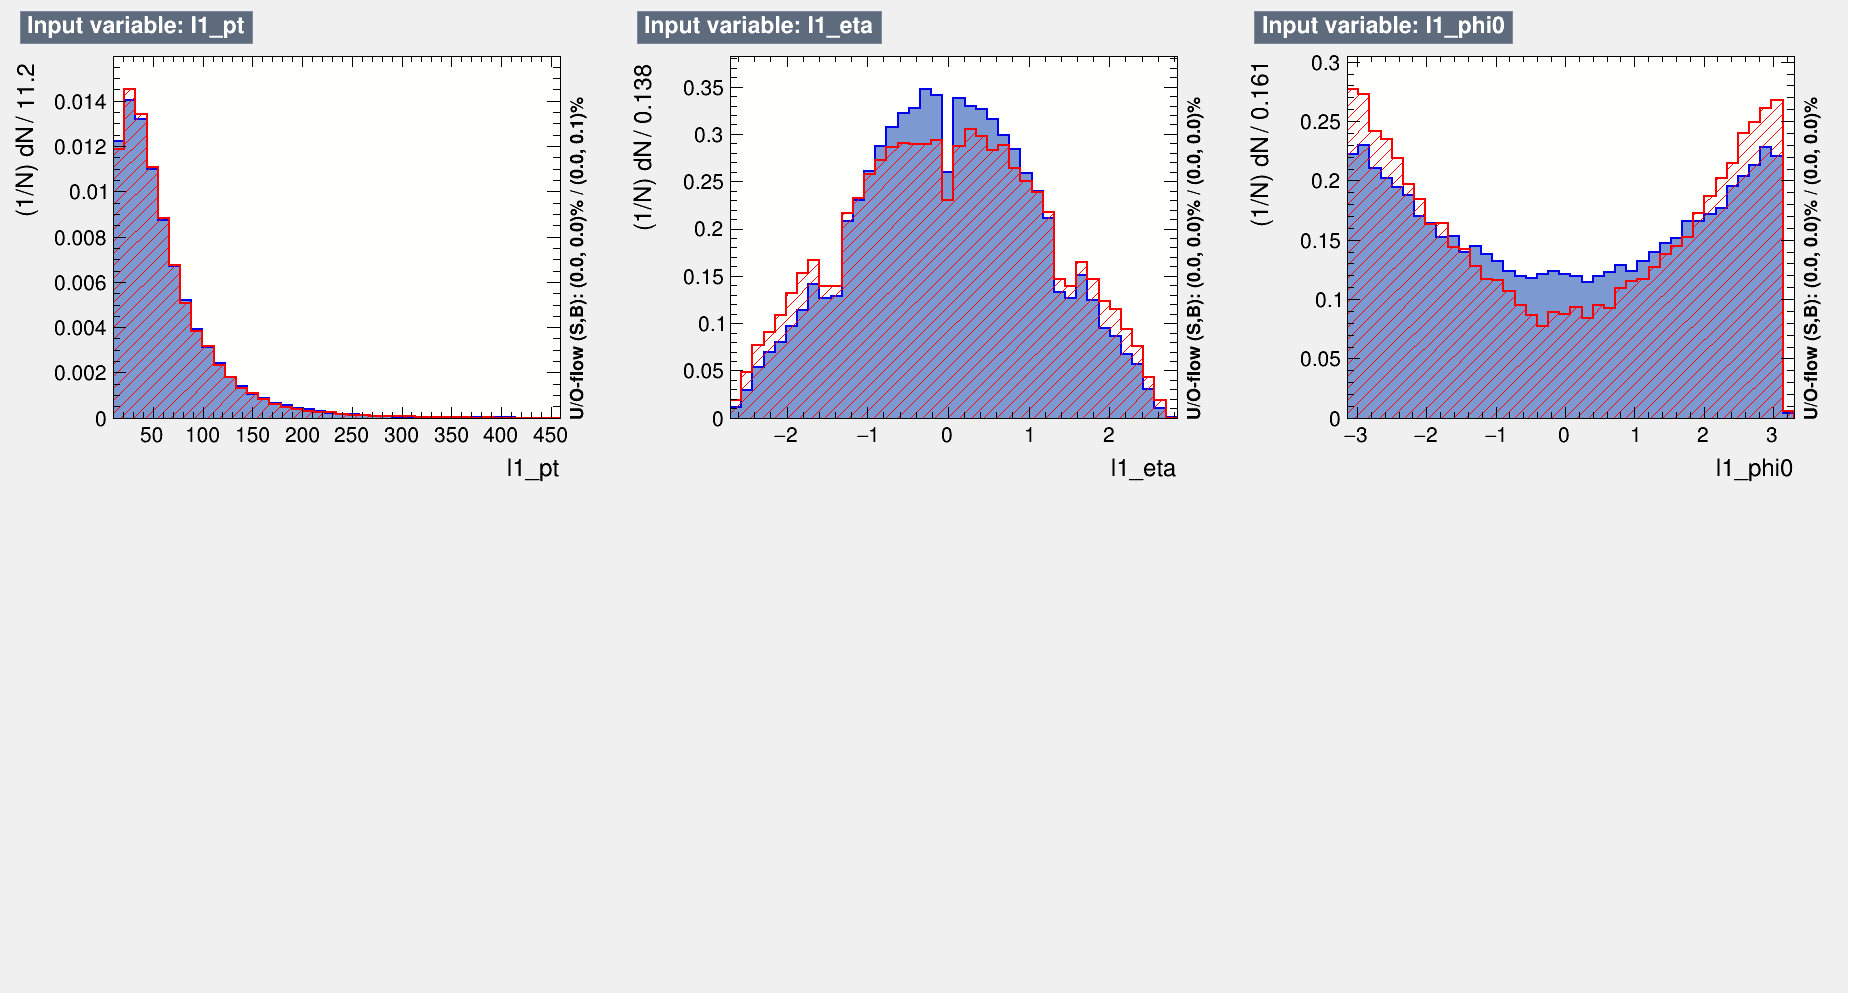
\includegraphics[width=0.62\textwidth]{figures/TMVABDTStudies/semilep-vbls4vec/semilep4vecvbls5.png}
  \caption{Normalized training variables for the 4-vector BDT, output by TMVA. CP-odd ttH is denoted as "signal" (blue); CP-even ttH is denoted as "background" (red). Variables shown are, from left to right, top row to bottom row: $p_{T}$ of leading lepton, $\eta$ of leading lepton, $\phi$ of leading lepton (measured with respect to the Higgs candidate)}
  \label{fig:semilep4vecvbls5}
\end{figure}
  
  
\subsection{Variable Optimization Studies, Nominal BDT, ttH and tH}

We use TMVA in order to perform a number of studies to investigate possible modifications to the nominal CPBDT, using CP-Odd $ttH+tH$ as signal and CP-Even $ttH+tH$ as background. For each study, we construct a different "Baseline" BDT, starting with the nominal CPBDT, then observe whether or not adding or altering a given variable will substantially impact the CPBDT performance (deeming a "substantial" impact to be one that increases $ttH$ + $tH$ Number-Counting Significance by at least 0.1$\sigma$, as gains below this threshold are likely to be noise).

We begin with a nominal BDT consisting of the following input variables and modify it in an iterative process, adding or removing variables depending on performance:

\begin{itemize}
\item $p_{T}$ (scaled by mass) and $\eta$ of the Higgs candidate
\item $p_{T}$, $\eta$, $\phi$ (wrt. Higgs candidate), and BDT score of the first and second reconstructed hadronic tops (see Section \ref{sec:topreco}). In the case where no second top is reconstructed, we use the $p_{T}$, $\eta$, and $\phi$ of the "hybrid" top.
\item Angles $\Delta\eta$ and $\Delta\phi$ between the top and the "hybrid" top.
\item Two-object invariant masses $m_{t1H}$, $m_{Hhy}$, and $m_{t1hy}$
\item The minimum $\Delta$R between a photon and a jet in the event
\end{itemize}

We come to the following conclusions:

\begin{itemize}
\item Adding the $p_{T}$, $\eta$, $\phi$, and pseudocontinuous b-tag score of the leading N jets in the event for N <= 6, where jets are ordered by $p_{T}$ does not substantially impact the significance (the largest significance gain from their inclusion was 0.07$\sigma$).

\item Adding the $p_{T}$, $\eta$, $\phi$, and pseudocontinuous b-tag score of the leading N jets in the event for N <= 6, where jets are ordered by b-tag score does not substantially impact the significance (the largest significance gain from their inclusion was approximately 0.06$\sigma$).

\item Changing $\Delta \eta (tops, Higgs)$ and $\Delta \phi (tops, Higgs)$ to $\Delta R (tops, Higgs)$ does not substantially impact the significance (the largest significance gain from this change was approximately 0.07$\sigma$).

\item Changing the choice of two or more of $M_{t1H}$, $M_{t1hy}$, or $M_{Hhy}$ does not substantially impact the significance (all combinations performed almost identically). We note that, because the BDT could in theory learn $M_{H}$ from combining more than two of these, we recommend only including two, the best-performing pair of which is $M_{t1hy}$ and $M_{t1H}$.

\item Adding the $p_{T}/M_{H}$, $\eta$, and $\phi$ of the two photons in the event does not substantially impact the significance (the largest significance gain from this change was approximately 0.02$\sigma$).

\item Adding the $p_{T}$, $\eta$, and $\phi$ of the two leading leptons in the event does not substantially impact the significance (the largest significance gain from this change was approximately 0.01$\sigma$).

\item Adding the missing transverse energy and its azimuthal angle does not substantially impact the significance  (the largest significance gain from their inclusion was 0.07$\sigma$).

\item Adding the minimum or second-smallest $\Delta$R between a photon and a jet in the event to the BDT does substantially impact the significance (the largest significance gain from their inclusion was 0.105$\sigma$ in the hadronic channel)
\end{itemize} 

We also recommend that, due to its potential dependence on $m_{H}$, $\cos$($\theta^{*}$) should not be included in the final CP-BDT.

\subsection{Dedicated CP-45 BDT Training}

We use TMVA to investigate the performance of a CP-BDT trained against the $\alpha = 45^{\circ}$ maximal-mixing CP signal sample, rather than the $\alpha = 90^{\circ}$ CP-odd signal sample used for the Nominal BDT.

As in the previous section, we begin with a different "Baseline" set of BDT variables, starting with the nominal CPBDT, then observe whether or not adding or altering a given variable will substantially impact the BDT performance (deeming a "substantial" impact to be one that increases the $ttH$ + $tH$ Number-Counting Significance by at least 0.1$\sigma$, as gains below this threshold are likely to be noise). Now, however, we use the Number-Counting Significance at $\alpha = 45^{\circ}$, rather than at $\alpha = 90^{\circ}$, as defined in Equation \ref{eq:nczcp} and Equation \ref{eq:ns}.

As in the previous section, we begin with a nominal $ttH+tH$ CPBDT consisting of the following input variables and modify it in an iterative process, adding or removing variables depending on performance:

\begin{itemize}
\item $p_{T}$ (scaled by mass) and $\eta$ of the Higgs candidate
\item $p_{T}$, $\eta$, $\phi$ (wrt. Higgs candidate), and BDT score of the first and second reconstructed hadronic tops (see Section \ref{sec:topreco}). In the case where no second top is reconstructed, we use the $p_{T}$, $\eta$, and $\phi$ of the "hybrid" top.
\item Angles $\Delta\eta$ and $\Delta\phi$ between the top and the "hybrid" top.
\item Two-object invariant masses $m_{t1H}$, $m_{Hhy}$, and $m_{t1hy}$
\item The minimum $\Delta$R between a photon and a jet in the event
\end{itemize}

We repeat the same set of tests as in the prior section and come to the same conclusions, namely, that we see no significant variations in the CP-45 significance by deviating from the nominal CPBDT architecture.

Using the BDT trained against the $\alpha = 45^{\circ}$ maximal-mixing CP signal sample, we observe an inclusive CP-Odd significance of 2.38 and a CP-45 Significance of 1.00 in the hadronic channel, as well as a CP-Odd significance of 1.79 and a CP-45 Significance of 0.78 in the leptonic channel.
This can be compared to the TMVA instantiation of the Nominal BDT trained against the CP-Odd signal sample, for which we observe an inclusive CP-Odd significance of 2.50 and a CP-45 Significance of 1.03 in the hadronic channel, as well as a CP-Odd significance of 1.85 and a CP-45 Significance of 0.77 in the leptonic channel.
For all four of these significance metrics, we find that the BDT trained against the CP-Odd signal sample performs comparably to the BDT trained against the $\alpha = 45^{\circ}$ maximal-mixing CP signal sample. Thus, using only only one $\alpha$-point as the BDT signal model rather than many is determined to be a robust choice for the analysis.
